\label{chap5}




In this chapter, the proposed model-based controller is tuned and verified in simulation and for experiments. First, the experimental set-up is presented, where the hardware, sensory devices and communication is detailed. Also, the design of digital filters is explained which are used for data acquisition. Then, the dynamic model is verified by a quasi-static analysis to obtain the actual actuator stiffness. Once the dynamic model is verified, a closed-loop step response is considered to tune the controller in simulation. Subsequently, the performance of this controller is analyzed for a reference trajectory. Next, the experimental case is considered. Again, the closed-loop step response is considered to tune the system. Finally, the results of a reference tracking problem conducted on the experimental set-up are presented. 


\section{Experimental set-up}

Figure \ref{fig5:setup} shows the experimental soft robot set-up as is present in the laboratory. The soft robot in the centre of the figure is mounted to the top of its supportive structure by threaded rods. To the soft robot itself, an LED and IMU carrier are connected. Furthermore, the two air inlets a the top of the soft robot can be seen. Each of these air inlets is in contact with an air pump as follows. Each air pump is attached to an air distribution manifold via a hose. This distribution manifold has three air outlets. To these outlets, a pressure sensor, air tank and actuator bellow are attached, respectively. To this end, silicone hoses with an inner diameter of 3 millimetres are used. To the tip of the actuator, a yellow LED is mounted that is used for optical tracking. This LED is glued to a connector that has been additively manufactured. The LED has an offset of 35 millimetres with respect to the tip of the actuator. This connector part also houses the IMU. This IMU is used to measure the rotation of the actuator's tip. Furthermore, a vision system is focused on the actuator. This vision system is programmed such that it can recognise and track the LED marker. The actual end-effector position can then be calculated using trigonometry using rotation and position data, see Appendix \ref{app:chap5} for this derivation.


\begin{figure}[H]
    \centering
    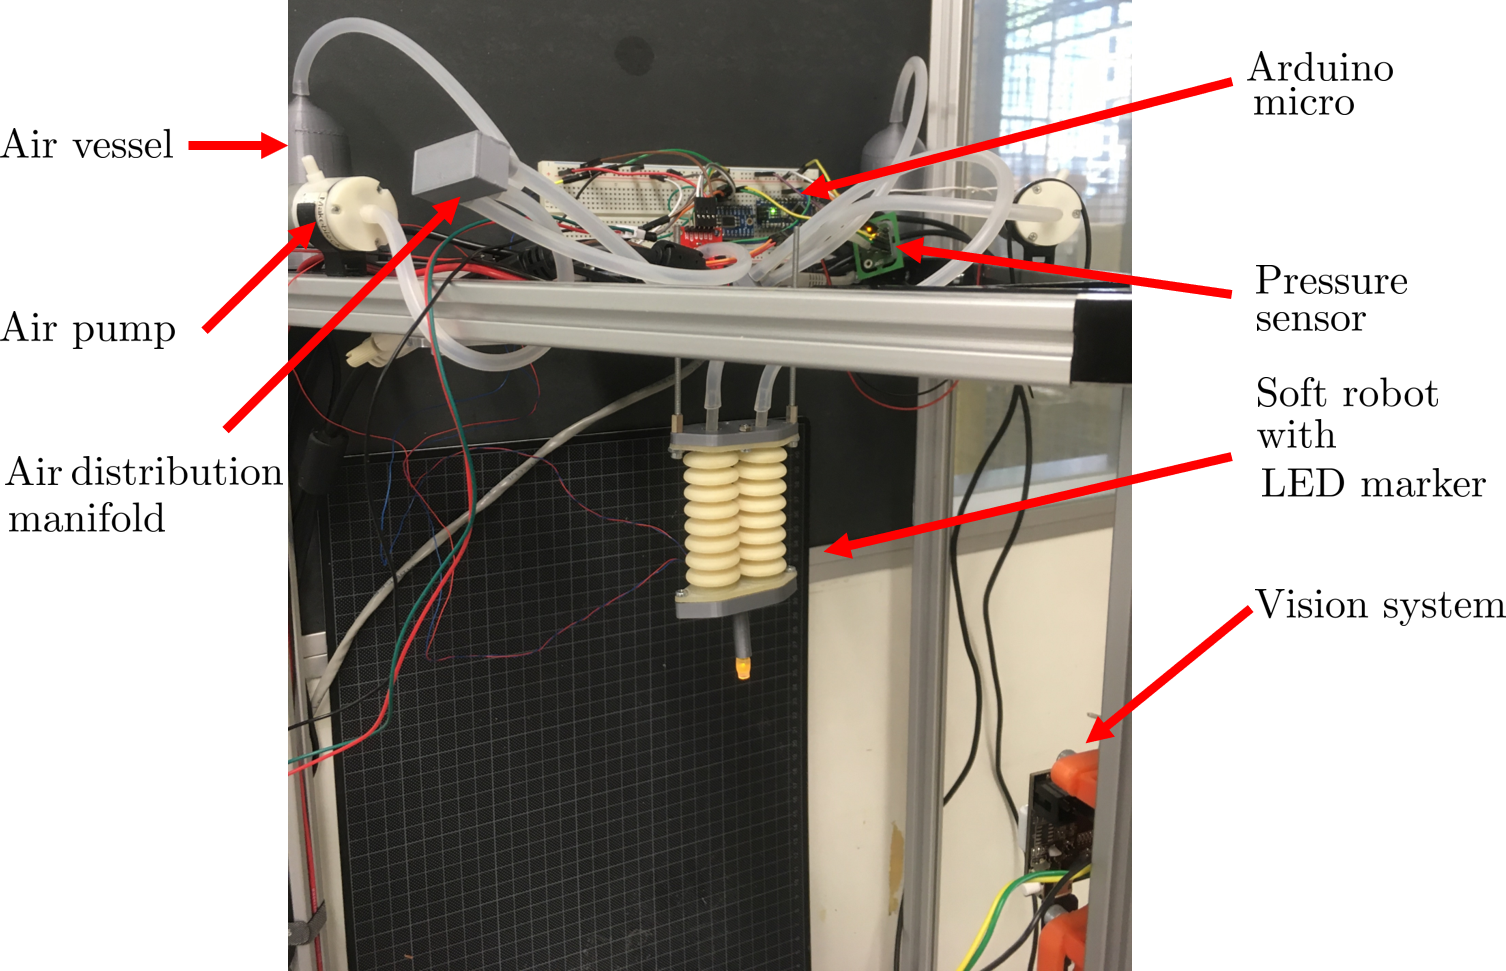
\includegraphics[width = \textwidth]{Figures/Chapter5/expsetup.png}
    \caption{Experimental setup of the soft robot.}
    \label{fig5:setup}
\end{figure}


The sensors described above, e.g. the IMU, two pressure sensors and optical tracking system are connected to an Arduino micro. This Arduino is connected to a Raspberry PI 3B+. The Arduino is used for data acquisition of the sensors. This includes the optical tracking system, two pressure sensors and the IMU. The maximum attained sample frequency of the Arduino is 40 Hz. On the Raspberry, the model-based controller and pressure controller are programmed. To the Raspberry, an ADC converter shield is mounted which can regulate the input to the air pumps. The Raspberry PI can receive sensor data and perform all necessary calculations at a frequency of 25 Hz. This is the maximum bandwidth frequency of the control system. This sampling frequency of 25 Hz might seem low compared to traditional robots. However, considering the slow system dynamics in the order of 1 Hz \cite{tawk2018bioinspired},\cite{HighBandwidthControl} this sampling frequency well suffices.


\subsection*{Digital filter design}

Since sensory devices are prone to measurement noise and disturbances, digital filters are implemented. For the IMU two different filters are applied. For the pressure and visions system, a single filter is used. 

For the IMU two filters are used to decrease noise and disturbances. First, the angle is filtered by a complementary filter, then a moving average filter is applied. The IMU houses an accelerometer, gyroscope and temperature sensor. The first two are necessary to determine rotation. The accelerometer can measure acceleration based on force, whereas the gyroscope allows for the measurement of rotational velocity. The output of both sensors is utilized to calculate rotation on all 3 axes. The accelerometer and gyroscope each have their deficits. The accelerometer exploits force measurements to determine acceleration. This also includes actuation forces, hence undesired high frequent pump dynamics influence the accelerometer readings. The gyroscope, on the other side, is prone to drift which becomes a problem over time. A complementary filter can be used to enhance angle calculations as this filter fuses gyroscopic data with acceleration data. To remove high-frequency noise the acceleration data is low-pass filtered, whereas gyroscope data is high-pass filtered. Therefore, the complementary filter can be described as, 

\begin{equation}
    \theta_{} = \delta \theta_{acc} + (1-\delta) \int_0^t \omega_{gyr} \hspace{2pt} ds    \hspace{25pt} \text{with}  \hspace{10pt} \theta_{acc} = \atantwo(a_y,a_x)
\end{equation}

where $\theta_{acc}$ is calculated from the measured accelerations $a_y$ and $a_x$ in the IMU's y-direction and x-direction, respectively. The rotational velocity $\omega_{gyr}$ is measured by the IMU's gyroscope. Parameter $\delta \in 0 < \delta < 1$ determines the relative importance between acceleration and gyroscope data. Since the angle readings with a complementary filter were not deemed satisfactory, a moving average filter is implemented. Solely using the complementary filter showed high amplitude oscillatory angle changes, whilst the tip velocity was near zero. The moving average filter reduces the amplitude of these oscillations as past angle data is used in the updated angle reading. The moving average filter is given as,

\begin{equation}
    \Bar{\theta}_k = \frac{1}{N_{IMU}}\sum_{i = 0} ^ {N_{IMU}-1} \theta_{k-i}
\end{equation}

where $\Bar{\theta}_k$ is the averaged output, $N$ the number of past samples to average and $\theta_k-i$ the past sample. It must be noted that both filters cause delays in the system. Therefore the tuning should be done carefully, as stability is not guaranteed.

The vision system which tracks the LED marker gives out its position data in pixels. These pixels are integer numbers, causing steps in the position measurement. To remove these steps and represent the mean position during a sampling instant the data is low-pass filtered. This casts the integers pixels to doubles, thereby expressing the position during a sample instant by its mean value. The description of the low-pass filter is identical to (\ref{eq4:lowpass}) and given as,

\begin{equation}
\bar{r}_{pixy,k} = \zeta_{pixy} r_{pixy,k} + (1-\zeta_{pixy})\bar{k}_{pixy,k-1}
\label{eq5:lowpass}
\end{equation}

where $\Bar{r}_{pixy,k}$ is the low-pass filtered position vector of the LED marker given in pixels. The sampled position vector is $r_{pixy,k}$ and $\bar{k}_{pixy,k-1}$ the previous filtered position. Parameter $\zeta$ determines the cut-off frequency of the low-pass filter. High values for $\zeta$ prioritize recent samples, whereas low values stress past LED positions. The pressure data is also low-pass filtered, following an identical procedure as the position data. 



\section{Dynamic Model verification}



To verify the dynamic model, the model's response is compared to a measured response of the actual set-up. For verification, the model and actual system are subjected to equivalent initial conditions and input. For a stable system, this is preferably a free oscillation, e.g. with input equal to zero. This allows isolating the soft robot dynamics from the pump dynamics as the latter are not excited. However, such a free oscillation can not be induced on the physical setup. An initial curvature or elongation can be induced, although not being perfectly in-plane. This slight out-of-plane initial condition causes the soft to oscillate out-of-plane, making the observed response nugatory for parameter estimation.


Another method to perform a parameter estimation is comparing the model and experimental response subjected to an identical input signal. A significant limitation of this method is the involved pump dynamics. The dynamics of the pumps are slow compared to those of the soft robot. This implies that accelerations and velocities are low. Therefore mass and damping properties of the system will be hard to identify using this method. However, this method is suitable to conclude on the modelled stiffness properties. Since the FEM analysis is conducted on a soft robot with thinner walls, the actual stiffness is expected to deviate from the modelled stiffness. It is expected that the soft robot used for experiments is stiffer for both elongation and curvature. 

This verification aims to find a linear scaling factor to scale the modelled non-linear stiffness to the actual stiffness. Since the accelerations and velocities are low the quasi-static modelled system can be expressed as,

\begin{equation}
   \underbrace{M(q) \Ddot{q}}_{\approx 0} + \underbrace{D \dot{q}}_{\approx 0} + K(q) q = Hp,
\end{equation}

where, for a steady state pressure, the modal coordinates only depend on the actual soft robot stiffness. It is assumed that the actual soft robotic stiffness can be formulated as $K(q)_{exp} = \alpha K(q)q$, with $\alpha \in \mathbb{R}^{2\times 2}$ a diagonal matrix to tune the modeled stiffness. Under the assumption that the measured pressure can be well described by a first-order model, the optimization to find $\alpha$ can be formulated as, 

\begin{equation}
    \min_{\alpha} (q_{exp} - q_{sim})^2 \hspace{10pt} s.t. \hspace{10pt} \alpha K(q) q_{sim} = Hp_{sim}
    \label{eq5:optalpha}
\end{equation}

where $q_{exp}$ are the experimentally obtained modal coordinates, and the $q_{sim}$ the modal coordinates in simulation. Recall the force mapping $H$ as given in Chapter \ref{chap3}. The simulated pressure is described by $p_{sim}$. The input to the air pumps is chosen as,

\begin{equation}
    V_1 =
\begin{cases}
0 & 0 < t < 2\\
V & 2 \leq t < 22\\
0 & 22 \leq t < 122\\
V & 122 \leq t < 142\\
0 & 142 \leq t < 180\\
\end{cases} \hspace{30pt} \text{and} \hspace{30pt}      V_2 =
\begin{cases}
0 & 0 \leq t < 82\\
V & 62 \leq t < 82\\
0 & 82 \leq t < 122\\
V & 122 \leq t < 142\\
0 & 142 \leq t < 180\\
\end{cases} ,
\end{equation}

where the two step inputs between 2 and 22 \& 42 and 62 seconds cause the soft robot to curve in positive and negative direction, respectively. Between 142 and 162 seconds, an equal volt input to both air pumps is supplied to induce an elongation. For this analysis, it was opted to use step inputs, since for these inputs accurate pressure models can be derived. This is beneficial when optimizing over $\alpha$, as errors in elongation and curvature are minimized as a cause of incorrect pressure models. The analysis is repeated for volt steps of 7, 9 and 11 Volts, respectively. For each air pump and volt input, the attained experimental pressure is fit to a first-order linear model. This pressure model is based on the step input inducing a curvature. The used first-order model to fit pressure is provided in Chapter \ref{chap3}. Deflation is not accounted for by this pressure model. 

The measured modal coordinates and results of the fitted stiffness are presented in Figure \ref{fig5:elong} and Figure \ref{fig5:kappa} for elongation and curvature, respectively. Instead of optimizing (\ref{eq5:optalpha}), the linear scaling for the stiffness curves have been obtained by iteratively running the dynamic model. Based on the outcomes of the steady-state elongation and curvature, $\alpha$ can be fitted. Of course, the optimization algorithm of (\ref{eq5:optalpha}) could have been utilized to find the scaling factors. However, the heavy computations result in exceptionally long simulation times. Therefore, this method was preferred, although being less accurate. Eventually, $\alpha$ was found to be equal to $\text{diag}([3.125,3])$. This implies that the modelled stiffness is around a factor 3 lower compared to the actual stiffness. The mass of the system is equal to $33.2$ grams. The damping properties were chosen as $D = \text{diag}([4e-5,2.5e-2])$. Furthermore, Figure \ref{fig5:p1} and \ref{fig5:p2} show the measured and simulated pressure. The pressure model describes the pressure for a curvature accurately. During the elongation, occurring between 120 and 140 seconds, the pressure model shows some deviation. Also, notice that the pumps do not reach equal steady-state pressure for equivalent volt input. This also results in curvature during the elongation phase, as can be seen in Figure \ref{fig5:kappa}. Most likely this is the deterioration of the pumps after extended use. 

\begin{figure}[H] 
    \begin{minipage}[b]{0.49\linewidth}
     \centering
    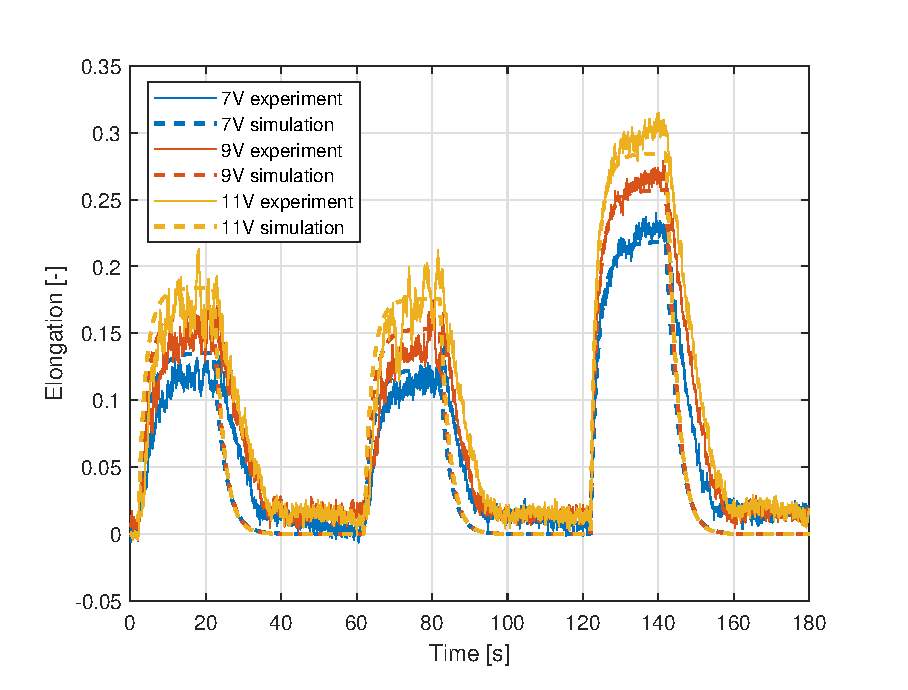
\includegraphics[width=\linewidth]{Figures/Chapter5/elongfit.eps} 
    \caption{Elongation for experiments (solid) and model (dotted) with for scaled stiffness $K_\epsilon$ } 
    \label{fig5:elong} 
       \end{minipage} 
    \begin{minipage}[b]{0.49\linewidth}
     \centering
    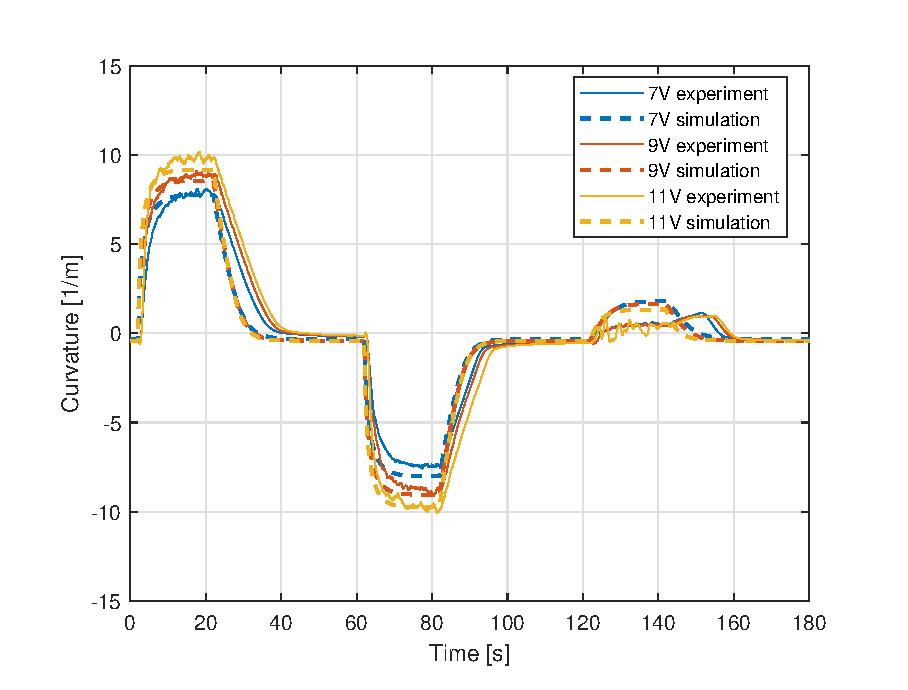
\includegraphics[width=\linewidth]{Figures/Chapter5/curvaturefit.eps} 
    \caption{Curvature for experiments (solid) and model (dotted) with for scaled stiffness $K_\kappa$ } 
    \label{fig5:kappa} 
    \end{minipage} 
\end{figure}

\begin{figure}[H] 
    \begin{minipage}[b]{0.49\linewidth}
     \centering
    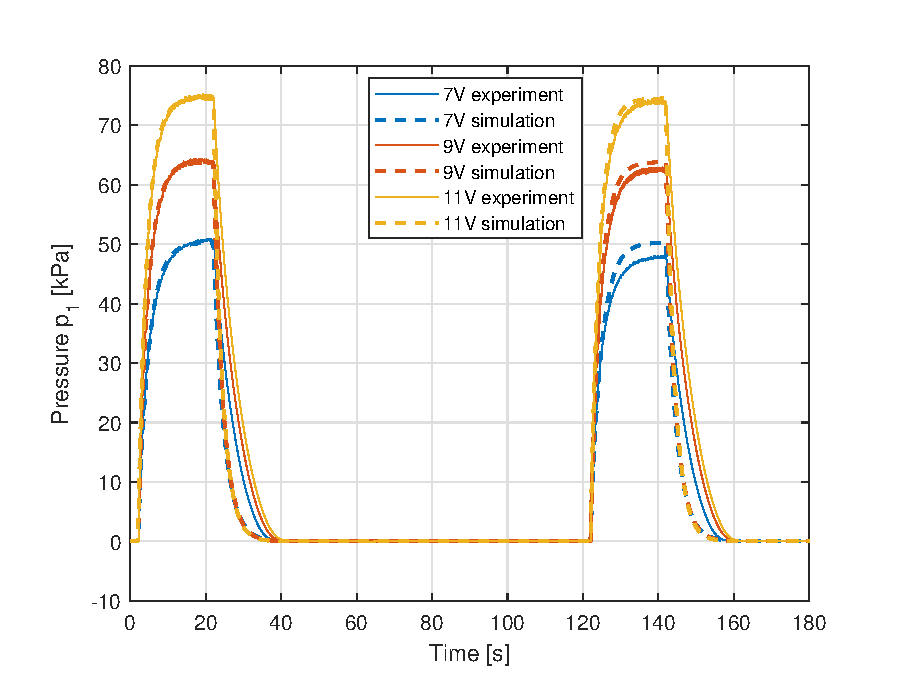
\includegraphics[width=\linewidth]{Figures/Chapter5/paramp1.eps} 
    \caption{Experimental and simulated pressure } 
    \label{fig5:p1} 
       \end{minipage} 
    \begin{minipage}[b]{0.49\linewidth}
     \centering
    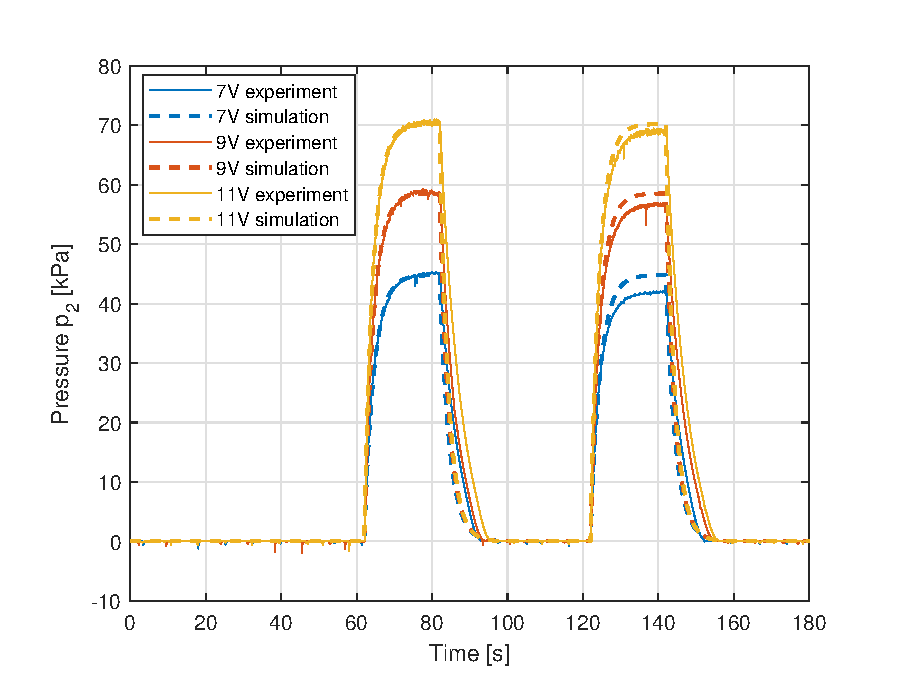
\includegraphics[width=\linewidth]{Figures/Chapter5/paramp2.eps} 
    \caption{Curvature for experiments and model with for scaled stiffness $K_\kappa$ } 
    \label{fig5:p2} 
    \end{minipage} 
\end{figure}




\section{Controller verification}

The controller as designed in Chapter \ref{chap4} is verified in simulation and experimentally. First, the controller will be verified on the developed dynamic model of the soft robot. The closed-loop response of the system to a step input is analyzed. This step input is also used for controller tuning. Subsequently, an ellipsoid reference signal is proposed to evaluate the tracking performance of the Jacobian controller in simulation. Then, the Jacobian controller is implemented on the experimental setup. The same closed-loop step response is considered for controller tuning. Additionally, the mirrored reference position is included, to verify if systems behaviour is similar. The achieved results and error performance are provided. Finally, the tracking performance of an ellipsoid reference signal is evaluated for the experimental set-up. 


\subsection*{Closed-loop step response in simulation}

To verify controller in simulation the closed-loop step response with a set-point $r_{set} = [-0.014,0.082]m$ is considered. This set-point demands the soft robot to curve and elongate, and therefore allows tuning all gains of the Jacobian controller. First, the tuning of the Jacobian controller and pressure controller is provided. Then the results of the step-response are presented and discussed. 

Since the effects of noise are omitted in the simulation, controller tuning is not as challenging as for the experimental case. The obtained controller gains are presented in Table \ref{tab5:gainssim}. First, the proportional gains $K_p$ are tuned, such that the control input stays below the saturation limit. As can be seen in the table, there is an order of magnitude difference between gains $K_{p,1}$ and $K_{p,2}$. This is caused by the input mapping as presented in Chapter \ref{chap3}. The moment and force mapping deviate approximately a factor 100. Since the inverse mapping is used to set the reference pressure, large $K_{p,1}$ gains result in erroneous pressure set points. Relative high integration gains are necessary to accelerate error reduction. The low-pass filter of the model-based controller is tuned to decrease high frequent oscillations. These oscillations are a result of the step input caused by the proportional gains at the beginning of the simulation. 



\begin{table}[H]
    \centering
    \begin{tabular}{|c|c|} \hline
     \textbf{Tuning Parameter}    & \textbf{Value}  \\ \hline
    $K_p$ & $\text{diag}([300,3000])$  \\ \hline
    $K_i$ & $\text{diag}([17500,17500])$  \\ \hline
    $K_{pp}$ & $\text{diag}([1,1])$  \\ \hline
    $K_{ip}$ & $\text{diag}([1,1])$ \\ \hline
    $\zeta$ & 0.01 \\ \hline
    \end{tabular}
    \caption{Controller gains used for step input in simulation}
    \label{tab5:gainssim}
\end{table}

\textcolor{red}{if one looks closely we can see a transition from an almost straight line, to a curved line during the first 0.2 seconds in the error response. This is something we have discussed but is not clear from this figure/tuning. Omit this behaviour or present a case here/Appendix?}

The results of the step response in the simulation are presented in Figure \ref{fig5:errorsim} to \ref{fig5:pressuresim}. The error response as a function of time is displayed in Figure \ref{fig5:errorelips}. It can be seen that the initial error in x and y-direction is 14 and 12 mm, respectively. For both errors, it takes about 16 seconds to reach 0 steady-state error. In the first 0.4 second an almost linear error decrease is observed, as an effect of the proportional gains. The error response then shows first order system behaviour. This is majorly because of the pump dynamics which act as low pass filters. Additionally, the low-pass filter of the model-based controller filters high frequent oscillations. Both factors result in smooth yet slow error convergence. Due to the low-pass filter, oscillations in the error signal are largely reduced. The observed eigen-frequencies for curvature and elongation are 40 and 130 Hz, respectively. This indicates that stiffness to mass ratio is higher than expected. Since soft robots generally have an eigen-frequency in the order of 1 Hz \cite{tawk2018bioinspired}. The root of this result is believed to be related to the mass approximation as presented in Chapter \ref{chap3}, since stiffness has been experimentally verified. 

\textcolor{red}{another figure with the Jacobian matrix entries as function of time?}



\begin{figure}[H]
    \centering
\begin{minipage}{0.5\textwidth}
        \centering
        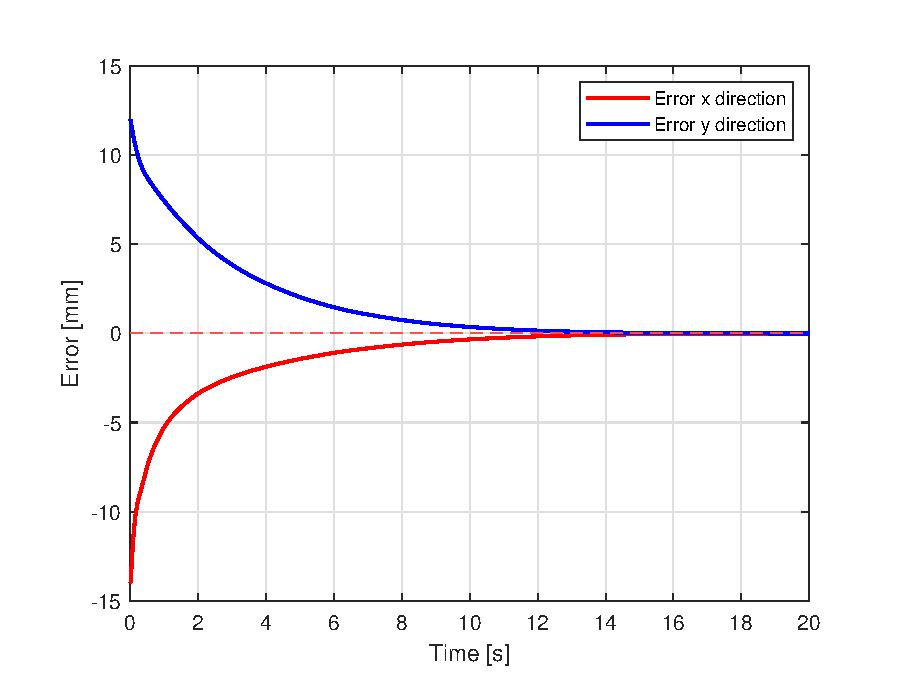
\includegraphics[width=\textwidth]{Figures/Chapter5/errorxysim.eps} 
        \caption{Error in x and y-direction as a function of time.}
        \label{fig5:errorsim}
    \end{minipage}\hfill
    \begin{minipage}{0.5\textwidth}
        \centering
        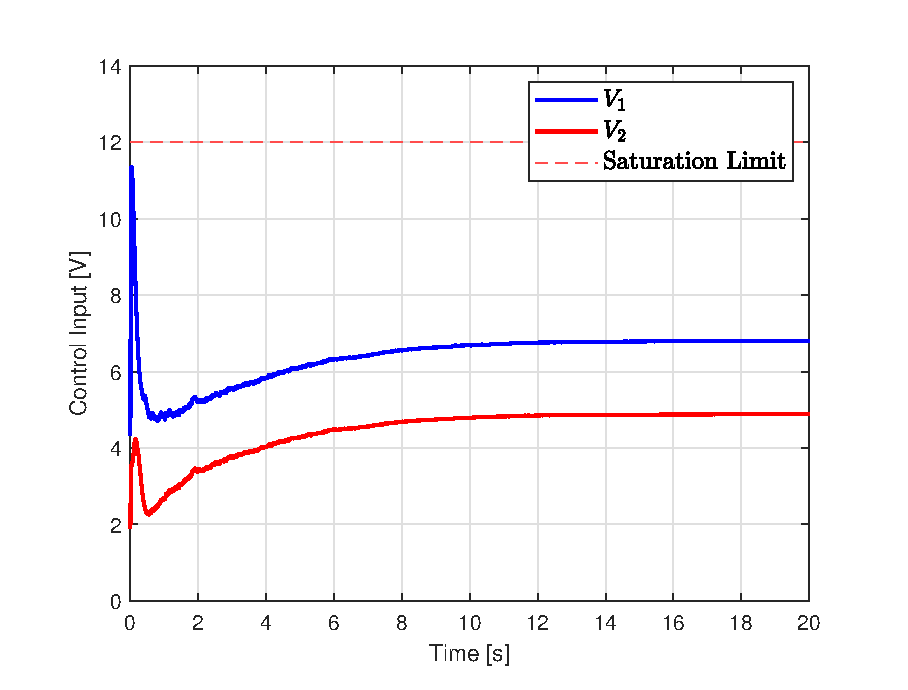
\includegraphics[width=\textwidth]{Figures/Chapter5/controlinputsim.eps} 
        \caption{Control input to the air pumps as a function of time}
        \label{fig5:controlinputsim}
    \end{minipage}
\begin{minipage}{0.5\textwidth}
        \centering
        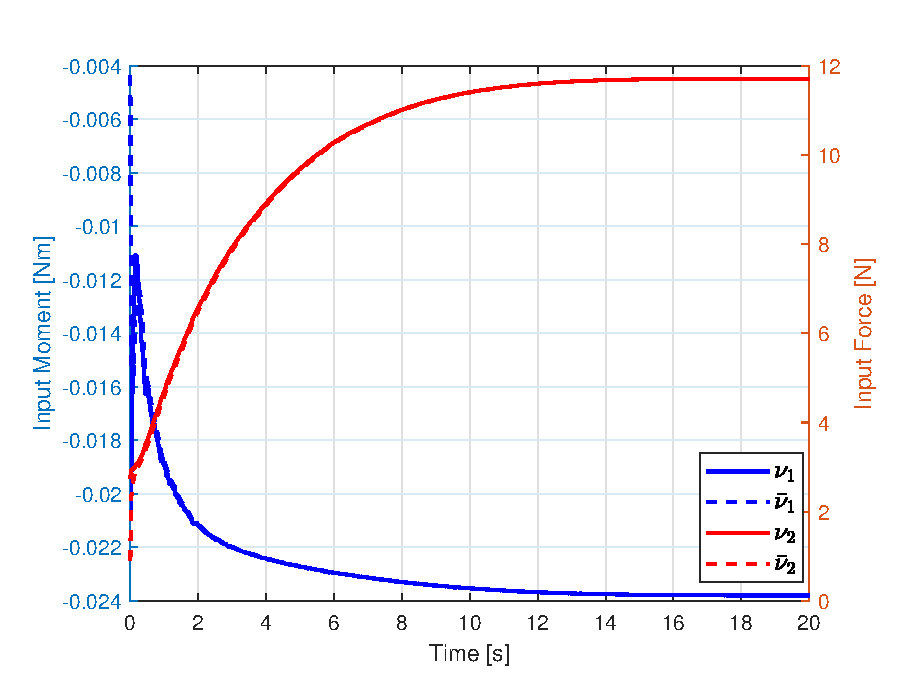
\includegraphics[width=\textwidth]{Figures/Chapter5/forcemomentsim.eps} 
        \caption{Input moment and force as determined by Jacobian controller. Solid line is unfiltered, dotted line is low-pass filtered}
        \label{fig5:inputsim}

    \end{minipage}\hfill
    \begin{minipage}{0.5\textwidth}
        \centering
        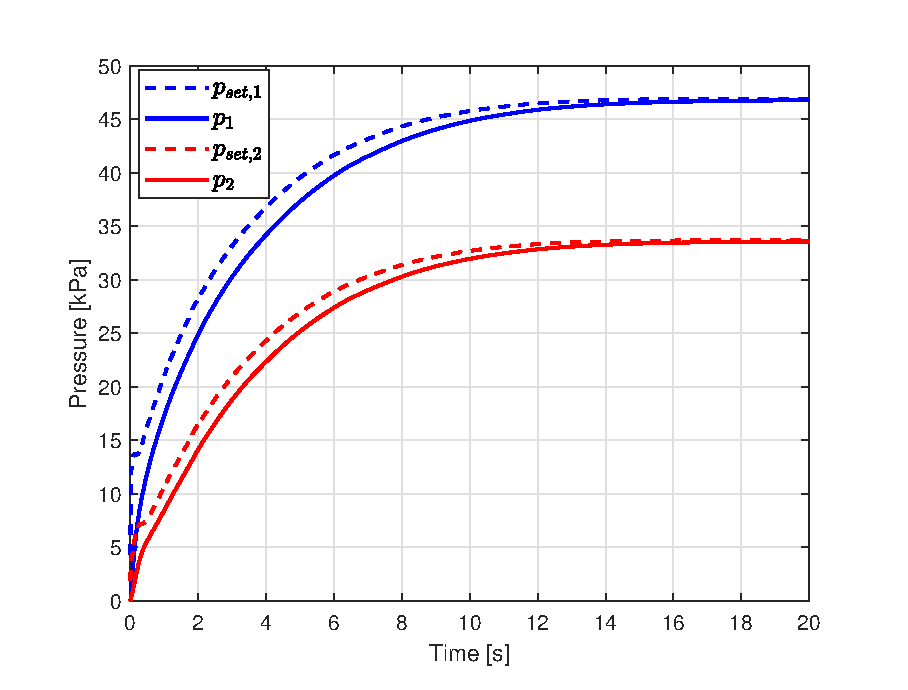
\includegraphics[width=\textwidth]{Figures/Chapter5/pressuresim.eps}
        \caption{Pressure response, dotted lines indicate reference pressure, solid lines are simulated pressures.}
        \label{fig5:pressuresim}
    \end{minipage}
\end{figure}




Figure \ref{fig5:pressuresim} shows the control input to the pump model. During the first seconds, the effects of high proportional gains can be observed. The input to the air pumps shows a peak, which quickly decreases the error. As an effect, to proportional gain decreases it's control effort. After 1 second, the integrator is mostly responsible for the error decrease, as control input to the air pumps slowly increases. Eventually, a steady input to the air pumps of 6.7 and 4.8 Volt is send. 

Figure \ref{fig5:controlinputsim} displays the input moment and force as determined by the model-based controller. The dotted lines show the low-pass filtered input which is send to the air pumps. It can be seen that although $\zeta$ is chosen just 0.01, the delay is low over the complete 20 second time window. The low-pass filter mostly acts during the first few seconds, where it attenuates high frequent input changes as a result of the excited system dynamics. 

Lastly, Figure \ref{fig5:pressuresim} shows the pressure response in simulation. The dotted lines indicate reference pressure, and the solid lines mark the simulated attained pressure. The figure shows that after 16 seconds a constant bellow pressure is obtained. This coincides with the error being zero after this time.



\subsection*{Closed-loop reference tracking in simulation}

Now the controller has been verified and tuned for a step response, its performance will be analyzed for a reference tracking problem. The reference tracking problem that is being considered in similar to the ellipsoid reference path of \cite{berkers}. Therefore, the outcomes this work can be well compared to the latter work. The ellipsoid reference path is described by the following equations,

\begin{equation}
    x_{ref} = \begin{cases} 
      0 &  t \leq t_1 \\
     \alpha \sin(2\pi \frac{t - t_1}{T_{ell}}) & t \leq T_{ell} + t_1 \\
     0 & t > T_{ell} + t_1
   \end{cases} 
\end{equation}

and,


\begin{equation}
    y_{ref} = \begin{cases} 
       y_{off} &  t \leq t_1 \\
     (y_{off} +\beta) -  \beta \cos(2\pi \frac{t - t_1}{T_{ell}}) & t \leq T_{ell} + t_1 \\
     y_{off} & t > T_{ell} + t_1
   \end{cases} 
\end{equation}

where it can be seen that during the first $t_1$ seconds the reference position is equal to offset $y_{off}$. Then, clockwise rotation occurs during $T_{ell}$ seconds in which the amplitude in the x-direction is $\alpha$, and the maximum elongation in y-direction is $y_{off} + 2\beta$. Once the ellipsoid has been completed, the reference signal is equal to its offset position. The values of these parameters are shown in Table \ref{tab5:refparams}. Since the controller has no feedforward control, and considering the slow dynamics of the system, $T_{ell}$ is chosen 400 seconds. The amplitudes, $\alpha$ and $\beta$ are comparable to the step inputs. The same controller parameters as obtained for the step-inputs in simulation are.


\begin{table}[H]
    \centering
    \caption{Reference tracking parameters}
    \begin{tabular}{|c|c|} \hline
   \textbf{Parameter}  & \textbf{Value [unit]} \\ \hline
    $t_1$ &   15 [s]  \\ 
    $y_{off}$ & 0.074 [mm] \\
    $\alpha$ & 13 [mm] \\
    $\beta$ & 7 [mm] \\
    $T_{ell}$ & 400 [s] \\ \hline
\end{tabular}
    \label{tab5:refparams}
\end{table}


The results of this ellipsoid reference in the x-y plane is shown in Figure \ref{fig5:xysim}. In this figure, the green crosses indicate the reference position at a given time. The red crosses mark the actual position at this time instant. It can be seen that a small delay is observed between the reference and the actual position. It can be seen that the controller is able to track the reference trajectory fairly accurate. A delay of about 2 seconds is observed between reference and actual position. Accounting for this 2 second delay, the RMS tracking errors during the ellipse is $e_{x,RMS} = 0.1489 mm^2$ and $e_{y,RMS} =0.0899 mm^2$ in x and y-direction, respectively. The error profiles are shown in Figure \ref{fig5:errorxyellipssim}. The first 15 seconds show a relative large error in y-direction as the soft robot is elongation to its offset position. The error that follows shows a sinusoidal shape, as is expected for a sinusoidal reference signal. The error response show two characteristics with respect to angle changes. At 105 seconds and at 325 seconds the error response shows a disturbance in both error signals. This is caused by the change in curvature rate. For the first quadrant the curvature is increasing, before it start decreasing. At 325 seconds the opposite occurs. A negative curvature rate switches to a positive curvature rate. This rate change affects the the Jacobian causing a disturbance on position level. At 217 seconds a similar disturbance can be observed. Again this is related to the curvature. At this time instant the curvature changes sign, again affecting the Jacobian and thus position. It should be noted that this disturbance is only present in $e_x$.


\begin{figure}[H] 
    \begin{minipage}[b]{0.49\linewidth}
     \centering
    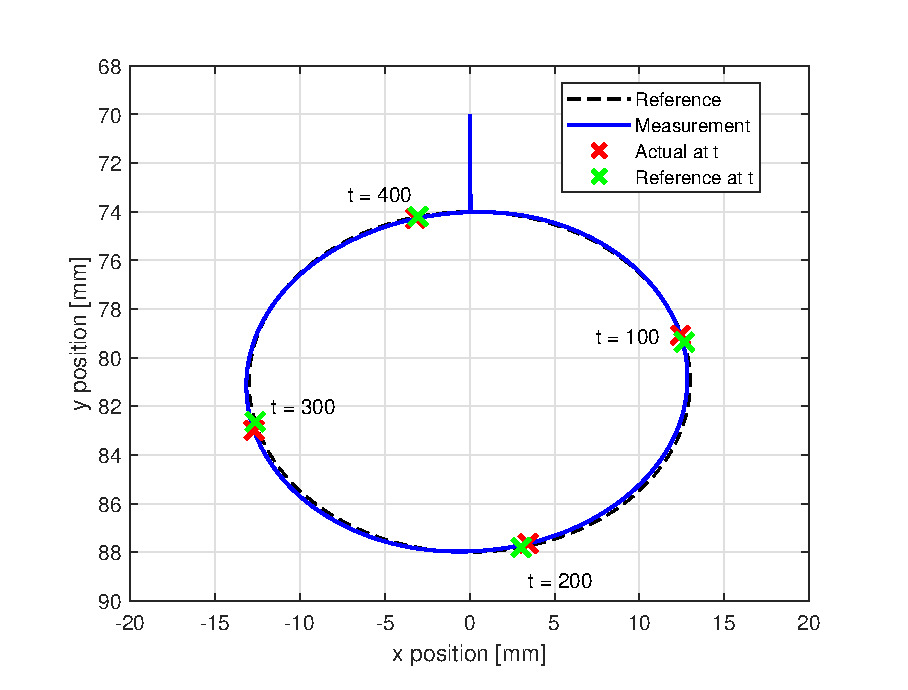
\includegraphics[width=\linewidth]{Figures/Chapter5/errorXYplaneTell400.eps} 
    \caption{Position in the x,y-plane for the ellipsoid reference path. } 
    \label{fig5:xysim} 
       \end{minipage} 
    \begin{minipage}[b]{0.49\linewidth}
     \centering
    \includegraphics[width=\linewidth]{Figures/Chapter5/errorxyTell400.eps} 
    \caption{Error in the x and y-direction as a function of time for an ellipsoid reference path.} 
    \label{fig5:errorxyellipssim} 
    \end{minipage} 
\end{figure}

Figure \ref{fig5:controlinputellipssim} shows the control input determined by the model-based controller, pressure response and control input to the simulated air pumps, respectively. The top figure shows a sinusoidal reference moment. Its extrema are situated at the times the x-displacement is highest. Likewise, the force input reaches a maximum when the maximum y-displacement is required. This coincides with the observations in the pressure response shown in the centre figure. Note that on this time scale the 2 second delay between reference moment and force and pressure can not be distinguished. The bottom figure shows the control input to the air pumps.


\begin{figure}[H]
    \centering
    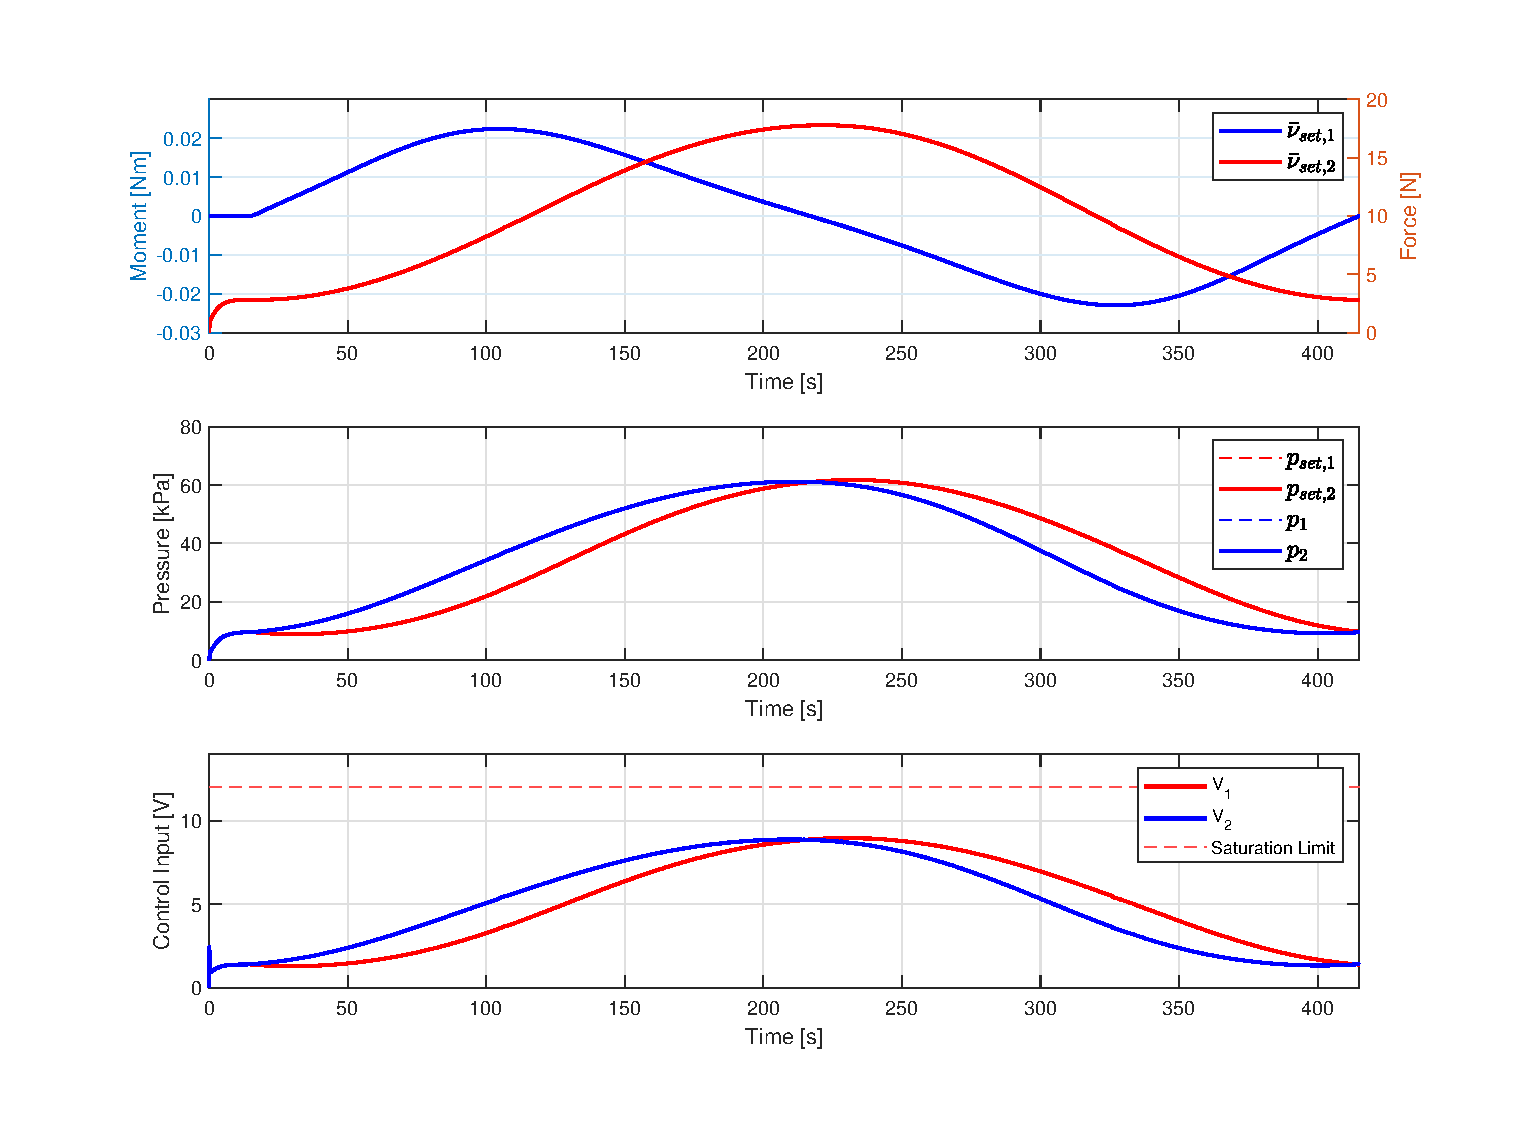
\includegraphics[width = \textwidth]{Figures/Chapter5/controlinputTell400.eps}
    \caption{\textbf{Top:} Input moment and force determined by model-based controller. \textbf{Middle:} Bellow pressure during ellipsoid reference tracking. \textbf{Bottom:} Control input send to the air pumps in simulation.}
    \label{fig5:controlinputellipssim}
\end{figure}

A concluding remark regarding the reference tracking in simulation. Given a sufficiently high $T_{ell}$ the controller is able to perform good tracking of the reference trajectory, in a noise free environment. Appendix \ref{app:chap5} supportive figures are shown regarding the entries of the Jacobian matrix over time while performing the reference tracking problem. Furthermore, a figure is provided showing the x,y position for an ellipsoid with $T_{ell}$ equal to 100 seconds. This figure supports the idea that feedforward control is necessary to enhance fast reference tracking.

\subsection*{Closed-loop step response in experiments}

Before the step response of the soft robot in experiments is provided, some adaptations to the input mapping are made. Furthermore, the controller tuning procedure of the experimental set-up is detailed. 

\subsection*{Revision of input mapping}

The accuracy of the obtained input mapping in Chapter \ref{chap3} as given by (\ref{eq3:H}) was questioned during the experiments. Recall that this mapping maps moment and force to individual bellow pressure. The obtained curvature and elongation stiffness's deviated an order of magnitude of 2 with each other. The original input mapping, increased the effort needed to tune the system. The large difference between force and moment mapping made the system susceptible to errors in pressure reference when tuning the gains of the model-based controller. Since the force mapping is approximately 100 times higher than the moment mapping, equivalent order of gains resulted in almost equal reference pressures for both bellows. This implies that the curvature stiffness is assumed to be underestimated. 

The input mapping has therefore been revised and was found as follows. First, the pressure controller gains are set as $K_{pp} =\text{diag}([1,1])$ and the integrator gain $K_{ip} = \text{diag}([0,0])$. In this way, the actual system pressure will never converge to the reference pressure. Subsequently, a set point is chosen for which the soft robot needs to elongate and curve. The proportional gain and integration gain are chosen such that steady-state is reached within a reasonable time. Eventually, the soft robot will move to its desired position set point, as the integrator action in the model-based controller will increase $\nu_{set}$. Once the reference position is reached, the input signal $\nu_{set}$ as determined with the old mapping remains constant. Furthermore, the actual system pressure in both bellows is known. Based on the pressures, and value of $\nu_{set}$ the entries of the input mapping can be redetermined. Following this procedure the revised input mapping was found as,

\begin{equation}
    H = \begin{bmatrix} 	0.0206 &  -0.0206 \\ 
	0.1808 & 0.1808 \end{bmatrix},
    \label{eq4:revisedH}
\end{equation}

where it can be seen that the moment to pressure mapping has increased by a factor 10. The force mapping was found equal order. A disadvantage of this method is that the newly obtained mapping matrix still depends on the initial mapping. Evidently, the $\nu_{set}$ is obtained with the old mapping. Therefore this mapping should be regarded as some sort of tuning mapping, defining the relative importance between force and moment. Hereto, the physical interpretation of reference force in Newton and moment in Newton-meter is lost to some extend. 

\subsection*{Experimental tuning procedure}


Table \ref{tab5:tuningcosiderations} shows the experimentally implemented tuning parameters together with its tuning consideration. The used parameters are found by iterative tuning and observing the system's response to a step input. The step input was chosen to be $r_{set} = [-0.014,0.082]m$. The tuning is done according to a procedure which is detailed.

Initially, the proportional gains $K_{pp}$ of the pressure controller are set as $\text{diag}([1,1])$. The integrator gains $K_{ip}$ are left as $\text{diag([0,0])}$. Subsequently, the low-pass filter gains on the sensors $\zeta_p$, $\zeta_{pixy}$ are set relatively high ($>0.9$), to minimize delays. Likewise, the sample amount of the moving average filter $N_{IMU}$ can be chosen low ($<5$). The complementary filter $\delta_{IMU}$ is taken initially as 0.02 \cite{compfilter}. These values allow passing through almost all recent data with a relatively small delay. Then the curvature set-point as $r_{set} = [0.014,0.082]^\top$ is selected. The proportional gains of the Jacobian controller $K_p$ are increased, such that the system does not saturate in the first few seconds of its response. Recall that the first entry $K_{p,1}$ affects the moment, and $K_{p,2}$ induces a force. Increasing the value of $K_{p,1}$ will result in a swing-like motion in the first seconds, caused by the initially large error in the x-direction. To minimize this behaviour gain $K_{p,1}$ should be chosen smaller than $K_{p,2}$. At this point, the integrator gain of the pressure controller $K_{ip}$ can be increased, to allow tracking of the pressure set point. Furthermore, the integrator gains $K_i$ can be tuned, these should be chosen relatively high to decrease position error relatively fast. The integrator gains are chosen too high when overshoot is observed. Since the system can not be actively deflated, and deflation rates are low, the integrator is not able to compensate well for overshoot. Next, the low-pass filter of the Jacobian controller $\zeta$ can be tuned. This parameter should be decreased to obtain a smooth input signal. At this point $\zeta_{pixy}$ can be tuned as well, to obtain a smoother position signal. Once the control input is smooth, the pressure response is considered. This response can be smoothed by decreasing the low-pass gain $\zeta_p$. Lastly, the sample amount $N_{IMU}$ of the moving average filter is tuned. This value should be tuned such that the angle settling time coincides with the error settling time. Once this procedure is completed, the system can be further fine-tuned to increase performance. Table \ref{tab5:tuningcosiderations} shows some guidelines and considerations whilst tuning the controller.

\newpage


\begin{table}[H]
    \centering
     \caption{Tuning considerations experimental tuning}
    \begin{tabular}{p{2.5cm} p{9cm} p{3cm}} \hline
      \textbf{Parameter}   & \textbf{Tuning  consideration} & \textbf{Value } \\ \hline
      $K_p$   &   $K_{p,1}$ affects curvature, whereas $K_{p,2}$ influences elongation. To decrease a swing like motion $K_{p,1} < K_{p,2}$. Motor saturation should be considered whilst tuning.   &  diag([$1750,3750$])            \\ \hline
      $K_i$   &   $K_{i,1}$ acts on the moment, to compensate for lower gain, this parameter can be increased. When the gains $K_p$ are set, $K_i$ can be increased up until error overshoot occurs.   &  diag([$6500,6250$])    \\ \hline
      $K_{pp}$   &  Is a scalar matrix due to assumed equal pump characters. It is not recommended to chose $K_p >1$ as this results in poor performance. Smaller values will result in a smoother volt input at the cost of performance.  &  diag([$1 ,1$])     \\ \hline
      $K_{ip}$   &  The integrator gains should be chosen such that system pressure tracks the reference pressure signal. If chosen too high, the system saturates the first seconds if used with high model-based control gains.    &  diag([$0.75,0.75$])    \\ \hline
      $\zeta$    &   This parameter allows to create smooth reference control input. A weigh-off is made between smoothness and delays. &  $0.08$  \\ \hline
      $\zeta_p$    &   This parameter has a major influence the control input. A smooth pressure reading will result in a smoother control input $V$. Low values will result in stability problems.   & $0.25$ $[-]$  \\ \hline
      $\zeta_{pixy}$    &  Since the vision system uses discretized pixel coordinates, a filter can be used to estimate position during a sample instant. Delays should be considered and minimized     & $0.25$   \\ \hline
      $N_{IMU}$    &  This value should be picked such that large oscillation in the angle readings are minimized, whilst reducing the delay as much as possible. & $35$   \\ \hline
      $\delta_{IMU}$    &  High values stress importance of accelerometer readings, low values emphasize gyroscopic data. Since the actuator forces affect accelerometer readings it is recommended not to pick $\delta_{IMU}$ too high.  & $0.08$  \\ \hline
    \end{tabular}
    \label{tab5:tuningcosiderations}
\end{table}



\subsection*{Step-response in experiments}


The performance of the designed controller in experiments is assessed by analyzing the system's step response. For the experimental verification two set-points are considered. As for the simulation, the first set-point is similar and equal to $r_{set} = [-0.014,0.082] m$. The second set-point is mirrored and given by $r_{set} = [0.014,0.082] m$. These set-points enable analyzing the movement in both Cartesian directions. Since it is assumed that the soft robot and pumps are perfectly symmetric, it is assumed that the system's response will be similar, only reversing the bellow pressures.

The system's error response as a function of time to set-point $r_{set} = [-0.014,0.082] m$ is given in Figure \ref{fig5:errorswingleft}. The figure shows the error signal in both directions. In the physical set-up, this set-point corresponds to a tip-movement to the left, hence ``left"  is used to address this set-point. A video is provided by clicking the link in the caption. The input send to the air pumps is presented in Figure \ref{fig5:inputswingleft}. Furthermore, Figure \ref{fig5:nuleft} shows control input $\nu$ as determined by the model-based controller. This figure shows the unfiltered, and low-pass filtered control input. Figure \ref{fig5:pleft} shows the bellow pressure of both bellows as solid lines. The dotted lines in this figure indicate reference pressure.


Figure \ref{fig5:stepleft} shows an initial error of 14 mm in x-direction, which corresponds to the set-point. As the initial error is largest, the proportional gain responds by increasing the volt input, as can be seen in the bottom figure. This results in a rapid decrease in error, causing a swing-like motion between 0.5 and 1.5 seconds. After 1.5 seconds the integrator takes over and the set-point is reached after 12 seconds. Considering a moment is necessary to enact displacement in the x-direction, the input moment as seen in Figure \ref{fig5:nuleft} is at a plateau of $-0.6 Nm$ after 12 seconds. 

Figure \ref{fig5:stepleft} also shows an initial error in the y-direction of 12 mm, which corresponds to the intended change in length. The swing-like motion can also be observed, which occurs at the same time as for the x-direction. The reference set-point in the y-direction is reached faster as it first hits the zero error line at around 6 seconds. This corresponds to the force set-point in Figure \ref{fig5:nuleft}, as the force at that time instant has reached a steady-state of around $13N$. 

The control input that is sent to the pumps is shown in Figure \ref{fig5:inputswingleft}. The first 1.5 seconds demonstrate the effect of the proportional gains. In this region, the error in both directions is largest. After around 10 seconds input $V_1$ and $V_2$ remain around the 5.3V and 8V, respectively. Figure \ref{fig5:pleft} shows the pressure in each bellow. It can be seen that the actual bellow pressure is tracking the pressure reference after 5 seconds, and remains close to this set point for the continuation of the experiment. The eventual steady-state pressure $p_1$ is equal to 51 kPa, the measured pressure $p_2$ is 21.3 kPa. In Appendix \ref{app:chap5} additional figures are presented, which include the response of $x,y$ and $\theta$, and the modal coordinates as a function of time as determined by the simplified inverse kinematics. 


\begin{figure}[H] 
    \begin{minipage}[b]{0.49\linewidth}
     \centering
    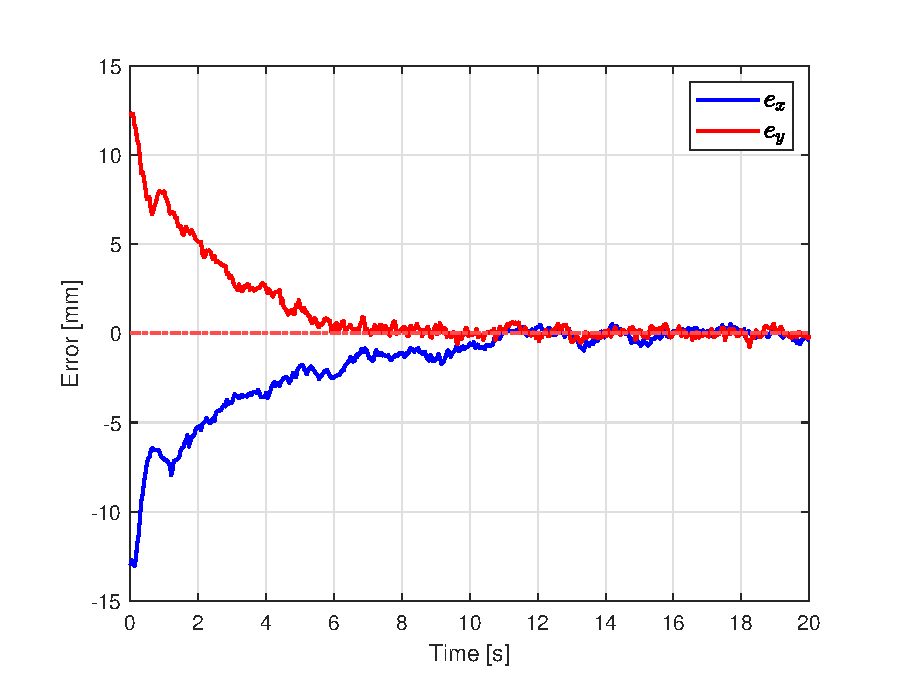
\includegraphics[width=\linewidth]{Figures/Chapter5/errorswingleftsquare.eps} 
    \caption{Error response in x and y-direction.Video provided at URL: \url{https://youtu.be/xz6EJKAM77Q}} 
    \label{fig5:errorswingleft} 
       \end{minipage} 
    \begin{minipage}[b]{0.49\linewidth}
     \centering
    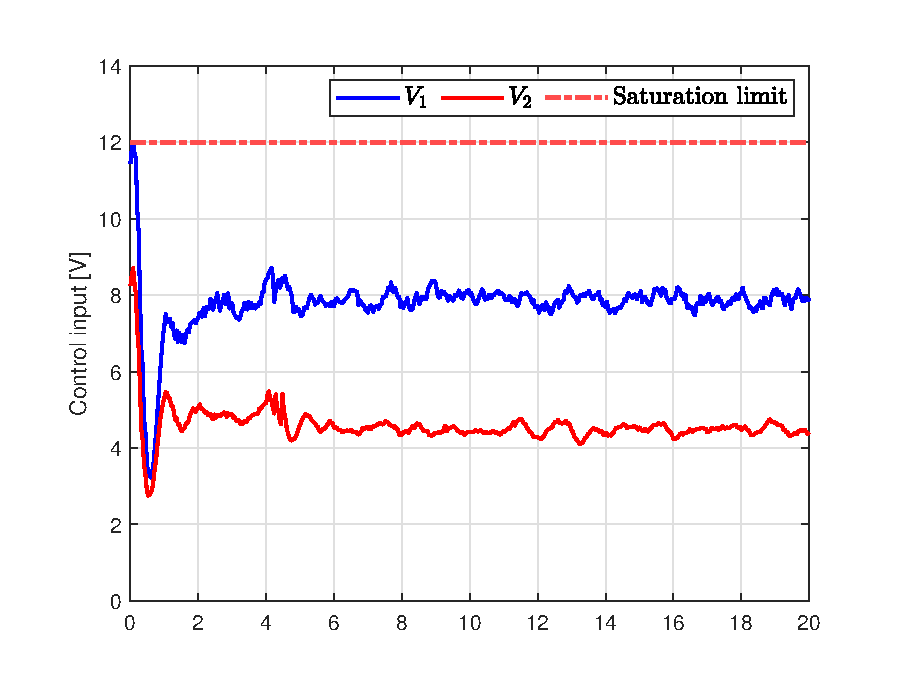
\includegraphics[width=\linewidth]{Figures/Chapter5/controlinputswingleft.eps} 
    \caption{Volt control input signal to the air pumps.} 
    \label{fig5:inputswingleft} 
    \end{minipage} 
\end{figure}



\begin{figure}[H] 
    \begin{minipage}[b]{0.49\linewidth}
     \centering
    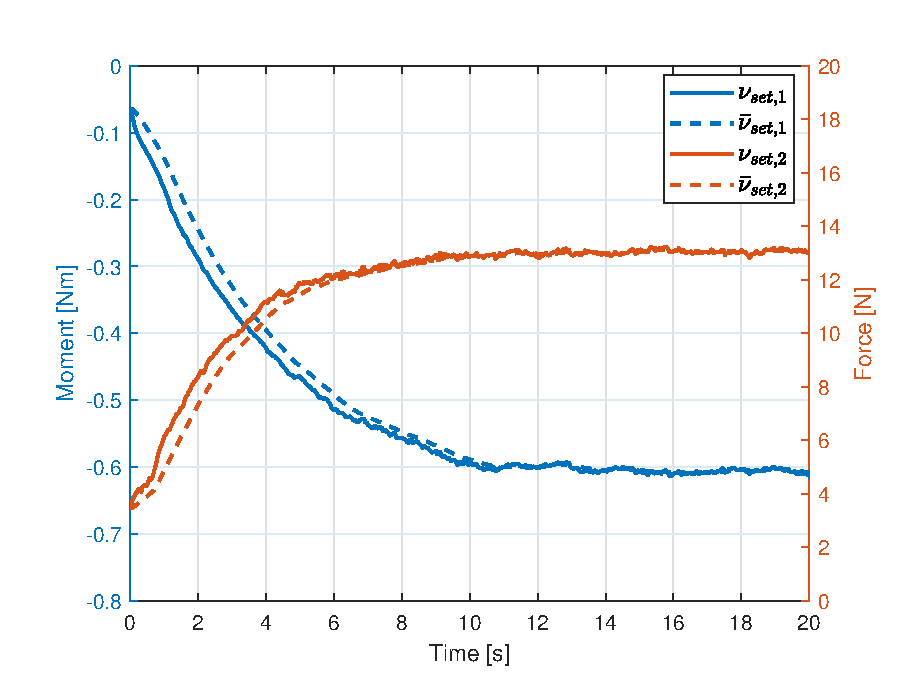
\includegraphics[width=\linewidth]{Figures/Chapter5/nuleft.eps} 
    \caption{Input moment and force as determined by Jacobian controller. Solid line is unfiltered input, dotted line low-pass filtered. } 
    \label{fig5:nuleft} 
       \end{minipage} 
    \begin{minipage}[b]{0.49\linewidth}
     \centering
    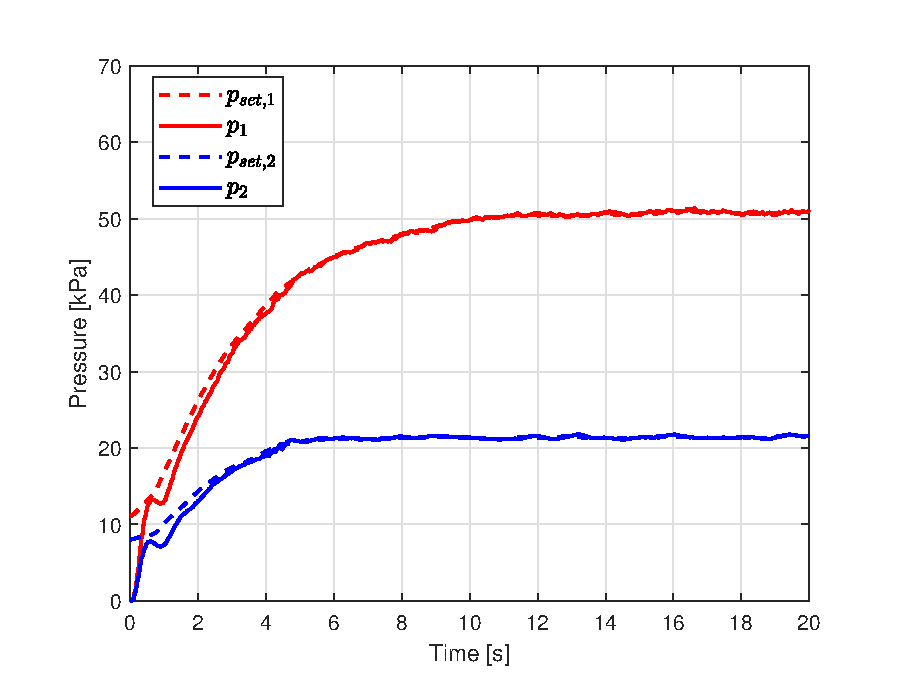
\includegraphics[width=\linewidth]{Figures/Chapter5/pressureleft.eps} 
    \caption{Pressure response, dotted lines indicate reference pressure, solid lines are measured pressures.} 
    \label{fig5:pleft} 
    \end{minipage} 
\end{figure}


As mentioned, the first set-point is mirrored to verify if the soft robot has equal characteristics when rotating in the opposite direction. For this step response the setpoint is $r_{set} = [0.014,0.082]^\top$. This set-point is denoted as the ``right".


The error response in both Cartesian direction is shown in Figure \ref{fig5:errorswingright}. Compared to the left set-point, this right set-point does not clearly show a swing during the first 2 seconds. Instead, a more gradual decrease in error is observed. After 13 seconds the zero error line is first crossed. From the input moment, as depicted in Figure \ref{fig5:nuright}, it can be seen that a steady-state is only reached after 20 seconds, at a value of $0.78 Nm$. Recalling, that a moment of $-0.6 Nm$ is necessary for the left set-point. Additionally, the bellow pressure $p_2$ reached a pressure of $60 kPa$ for the right setpoint, whilst for the left the set-point this was $51 kPa$. The reason for the observed behaviour remains inconclusively. A likely explanation are unequal pump characteristics caused by degradation of the valves. Or possibly, the material properties of the actuator are not equal throughout the soft robot. The error in y-direction for the right set-point shows similar behaviour as for the left set-point. The settling time is around 10 seconds which is 2 seconds more when compared to the first set-point. This can also be seen from force input in Figure \ref{fig5:nuright} which reaches a steady-state force of $15 N$.

Figure \ref{fig5:inputswingright} shows the control volt send to the air pumps. The observed response is similar to the previous set-point. The input during the first 1.5 seconds is initiated by the proportional action. After 1.5 seconds, the integrator action becomes dominant over the proportional gain. Eventually the control input $V_1$ and $V_2$ stay close to 4.3 and 9.5 V, respectively. This voltage is higher compared to the left set-point, as the stiffness in this rotational directions seems to be higher. The control input to the motor also contains higher amplitude changes, which are linked to the noise on the pressure signal. Figure \ref{fig3:pump_dynamics_adapted} in Chapter \ref{chap3} showed that for higher pressures the noise floor increases. The noise effects can be observed in the controller input. To decrease these effects a low-pass filter on the pressure controller could be implemented, or the cut-off frequency of the low-pass filter on the pressure data could be decreased. However, both actions increase delays in the system which could cause stability problems.

Additional figures regarding the measured $x,y$ and $\theta$ position and modal coordinates can be found in Appendix \ref{app:chap5}.




\begin{figure}[H] 
    \begin{minipage}[b]{0.49\linewidth}
     \centering
    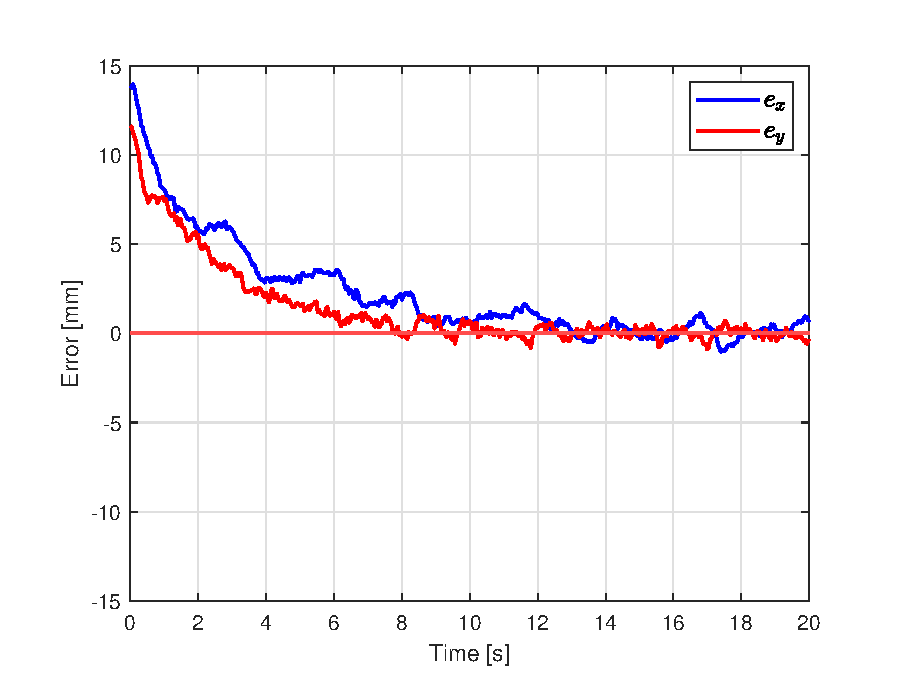
\includegraphics[width=\linewidth]{Figures/Chapter5/errorswingrightsquare.eps} 
    \caption{Error response in x and y-direction.Video provided at URL: \url{https://youtu.be/osywb0OYl7U}} 
    \label{fig5:errorswingright} 
       \end{minipage} 
    \begin{minipage}[b]{0.49\linewidth}
     \centering
    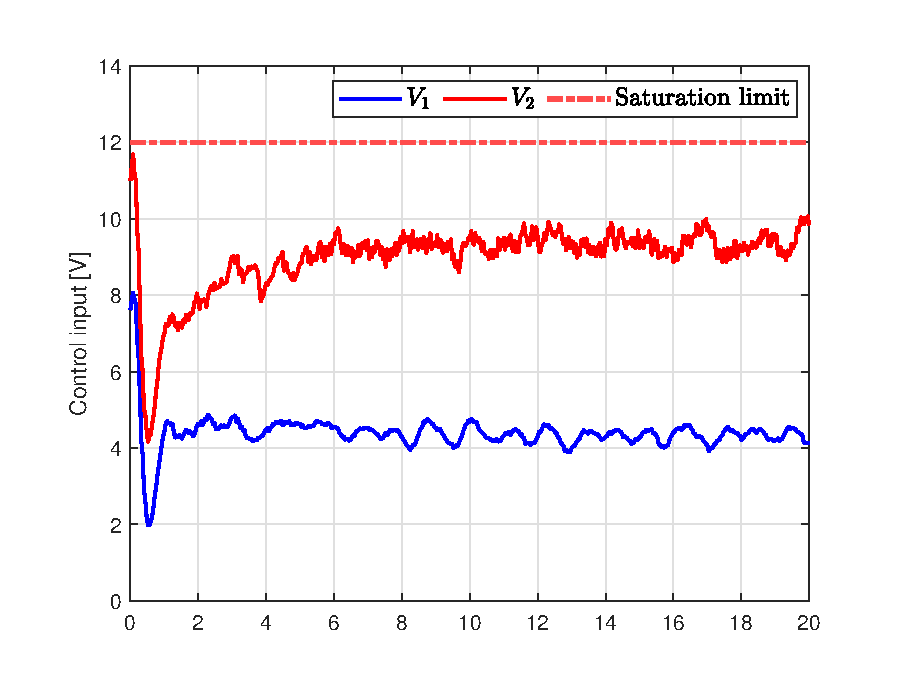
\includegraphics[width=\linewidth]{Figures/Chapter5/controlinputswingright.eps} 
    \caption{Volt control input signal to the air pumps.} 
    \label{fig5:inputswingright} 
    \end{minipage} 
\end{figure}



\begin{figure}[H] 
    \begin{minipage}[b]{0.49\linewidth}
     \centering
    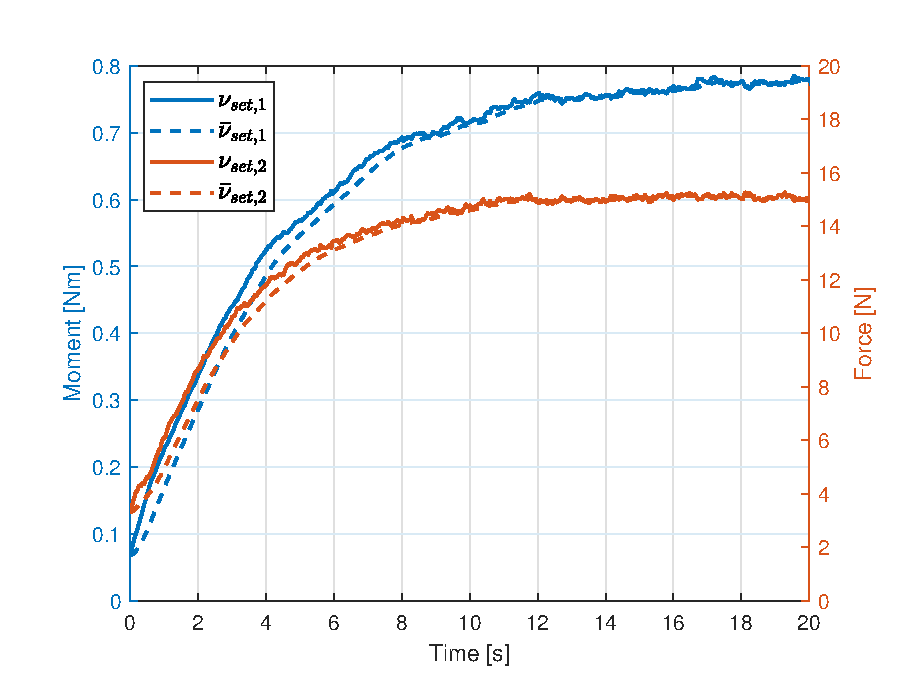
\includegraphics[width=\linewidth]{Figures/Chapter5/nuright.eps} 
    \caption{Input moment and force as determined by Jacobian controller. Solid line is unfiltered input, dotted line low-pass filtered. } 
    \label{fig5:nuright} 
       \end{minipage} 
    \begin{minipage}[b]{0.49\linewidth}
     \centering
    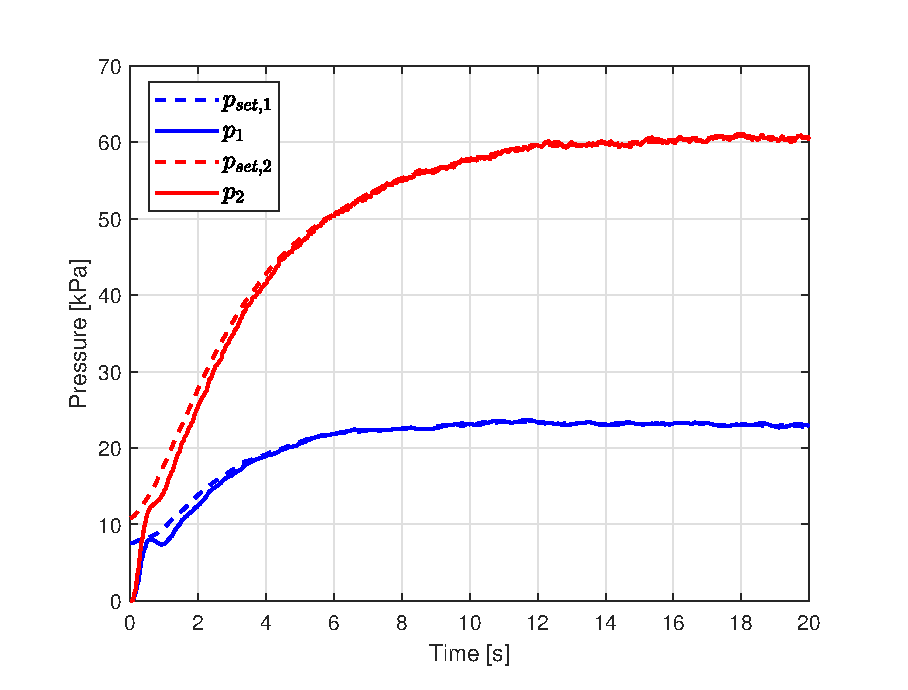
\includegraphics[width=\linewidth]{Figures/Chapter5/pressureright.eps} 
    \caption{Pressure response, dotted lines indicate reference pressure, solid lines are measured pressures.} 
    \label{fig5:pright} 
    \end{minipage} 
\end{figure}



For both set-points the Root-Means-Square (RMS) error is analysed after the control input $\nu$ reaches its steady-state control input. To this end, an experiment for more than 20 seconds is carried out. The obtained error values are presented in Table \ref{tab:RMSerrors}. It can be seen that the RMS error for the right set-point is larger compared to the left set-point. The cause of this problem is related to the stiffness properties of the actuator. The curvature stiffness for positive and negative rotation is not uniform. This could be related to manufacturing tolerances, e.g. the material thickness of both bellows is not equal. Other possibilities can relate to the elastomer itself, e.g. exposure time of the laser or the time interval between each printed layer. 



\begin{table}[H]
    \centering
    \caption{RMS error after 15 seconds}
    \begin{tabular}{|c|c|c|} \hline
     Set point $[x,y]^\top$    & $e_{RMS,x}$ $mm^2$  &  $e_{RMS,y}$ $mm^2$  \\ \hline
    Left $r_{set}= [-0.014,0.082]^\top$     & 2.6034e-04  & 2.2644e-04 \\ \hline
    Right $r_{set}= [0.014,0.082]^\top$  &  3.2692e-04 &   2.6577e-04\\ \hline
    \end{tabular}
    \label{tab:RMSerrors}
\end{table}



\subsection{Closed-loop reference tracking in experiments}

To evaluate the performance of the controller during a reference tracking problem the same reference signa. The equations describing this ellipsoid as function of time are given as,

\begin{equation}
    x_{ref} = \begin{cases} 
      0 &  t \leq t_1 \\
     \alpha \sin(2\pi \frac{t - t_1}{T_{ell}}) & t \leq T_{ell} + t_1 \\
     0 & t > T_{ell} + t_1
   \end{cases} 
\end{equation}

and,


\begin{equation}
    y_{ref} = \begin{cases} 
      \frac{(y_{off} - L) t}{t_1} + L&  t \leq t_1 \\
     (y_{off} +\beta) -  \beta \cos(2\pi \frac{t - t_1}{T_{ell}}) & t \leq T_{ell} + t_1 \\
     y_{off} & t > T_{ell} + t_1
   \end{cases} 
\end{equation}


where it can be seen that during the first $t_1$ seconds the reference position linearly increases to an offset $y_{off}$. Then, clockwise rotation occurs during $T_{ell}$ seconds in which the amplitude in the x-direction is $\alpha$, and the maximum elongation in y-direction is $y_{off} + 2\beta$. Once the ellipsoid has been completed, the reference signal is equal to its offset position. The values of these parameters are shown in Table \ref{tab5:refparams}. Since the controller has no feedforward control, and considering the slow dynamics of the system, $T_{ell}$ is chosen 100 seconds. The amplitudes, $\alpha$ and $\beta$ are comparable to the set-points presented in the previous section. The same controller parameters are used as for the set-point regulation experiments.


\begin{table}[H]
    \centering
    \caption{Reference tracking parameters}
    \begin{tabular}{|c|c|} \hline
   \textbf{Parameter}  & \textbf{Value [unit]} \\ \hline
    $t_1$ &   15 [s]  \\ 
    $y_{off}$ & 0.074 [mm] \\
    $\alpha$ & 13 [mm] \\
    $\beta$ & 7 [mm] \\
    $T_{ell}$ & 100 [s] \\ \hline
\end{tabular}
    \label{tab5:refparams}
\end{table}

The results of the above reference trajectory a plotted in Figure \ref{fig5:xyelips}. This figure shows the position in the x,y plane as a solid blue line, whereas the reference is plotted as a dotted black line. Additionally, green crosses mark the reference position at a given time, whereas red crosses mark the actual position at a given time. It can be seen that the actual position is lagging behind the reference position. For reference positions in the lower halve of the ellips is seems that the delay is larger compared to the upper halve. This phenomena can be explained by the fact that the system can not actively deflate. 
Low-pass filtering of the reference signal only results in a delay for the reference signal of around 0.5 seconds. 


This phenomenon can partly be explained by the low-pass filtering of the control input, which limits rapid changes in control input. Another explanation is the low-pass filtering of the position data as perceived by the vision system. To decrease the effect of the delay caused by the model-based controller, $T_{ell}$ can be further increased. The delays initiated by the vision system can be decreased by increasing cut-off frequency of its low-pass filter. However, this will effect the position readings as it raises noise levels. Figure \ref{fig5:errorelips} shows the error signal in x and y-direction for the reference tracking problem. Since the system is delayed, the position error as function of time is 

Part of this phenomenon can be explained by the low-pass filter in the model-based controller. This low-pass filter prevents rapid changes in control input

. The control input is determined based on the actual position and desired position. For a reference tracking problem both set-point and actual position are time dependent, whereas for the step-response the s
\
as response to a position error. Initially, this low-pass filter reduces  Therefore the error response as shown on the right-hand side of Figure \ref{fig5:errorellips} is not an accurate representation of the soft robot's capabilities. If the error signal
\textbf{when experiment has been }




\begin{figure}[H] 
    \begin{minipage}[b]{0.49\linewidth}
    \centering
    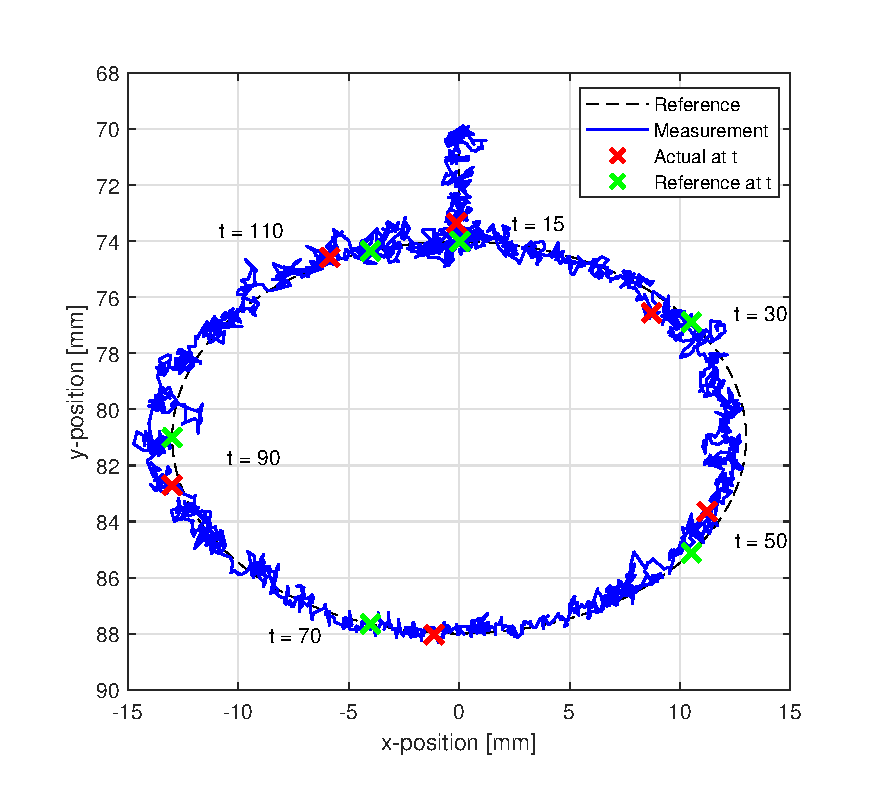
\includegraphics[width = \textwidth]{Figures/Chapter5/xy.eps}
    \caption{Position in the x,y-plane for the ellipsoid reference path. Video provided at URL: \url{https://youtu.be/8hYWhlwnYkY}}
    \label{fig5:xyelips}
       \end{minipage} 
    \begin{minipage}[b]{0.49\linewidth}
    \centering
    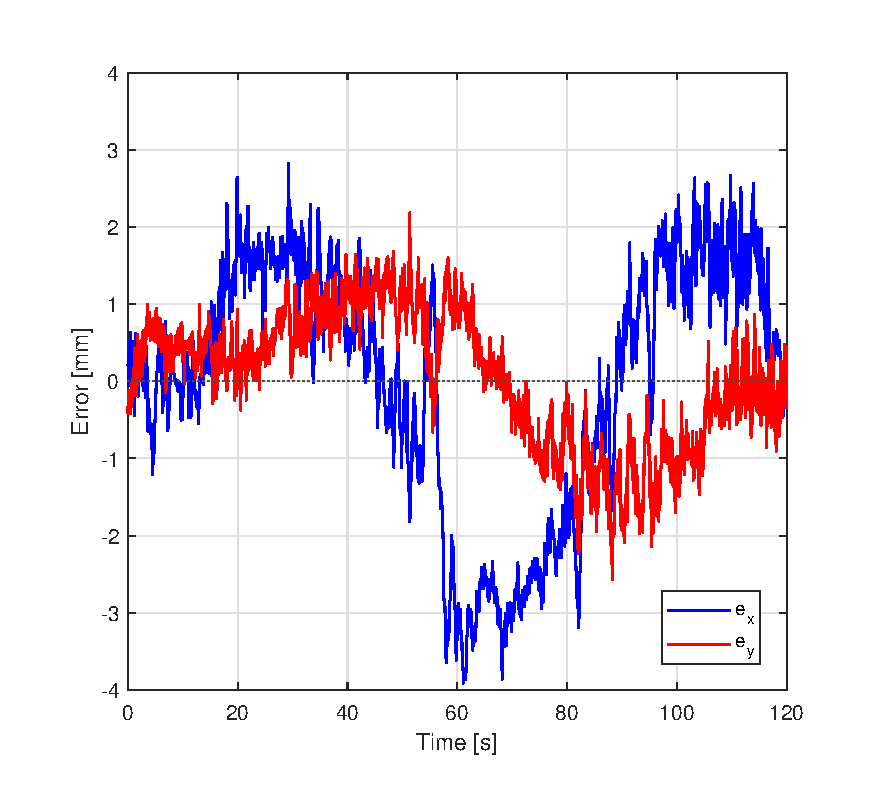
\includegraphics[width = \textwidth]{Figures/Chapter5/errorxy.eps}
    \caption{Error in the x and y-direction as a function of time for an ellipsoid reference path.}
    \hspace{10pt}
    \label{fig5:errorelips}
    \end{minipage} 
\end{figure}



Another observation is the high-frequent noise in the position measurement. During the experiments, these vibrations of the soft robot can be seen. The origin of this noise are related to the dynamics of the air pumps. The bottom figure in Figure \ref{fig5:controlellips}, shows the control input to the air pumps. This figure shows that especially in regions where the volt input approaches saturation levels large-amplitude volt changes occur. This coincides with the pressure step response as presented in Chapter \ref{chap3}, which showed increasing noise levels for pressure increases. Although the pressure data is low-pass filtered, spikes in the volt control input still occur. 


\begin{figure}[H]
    \centering
    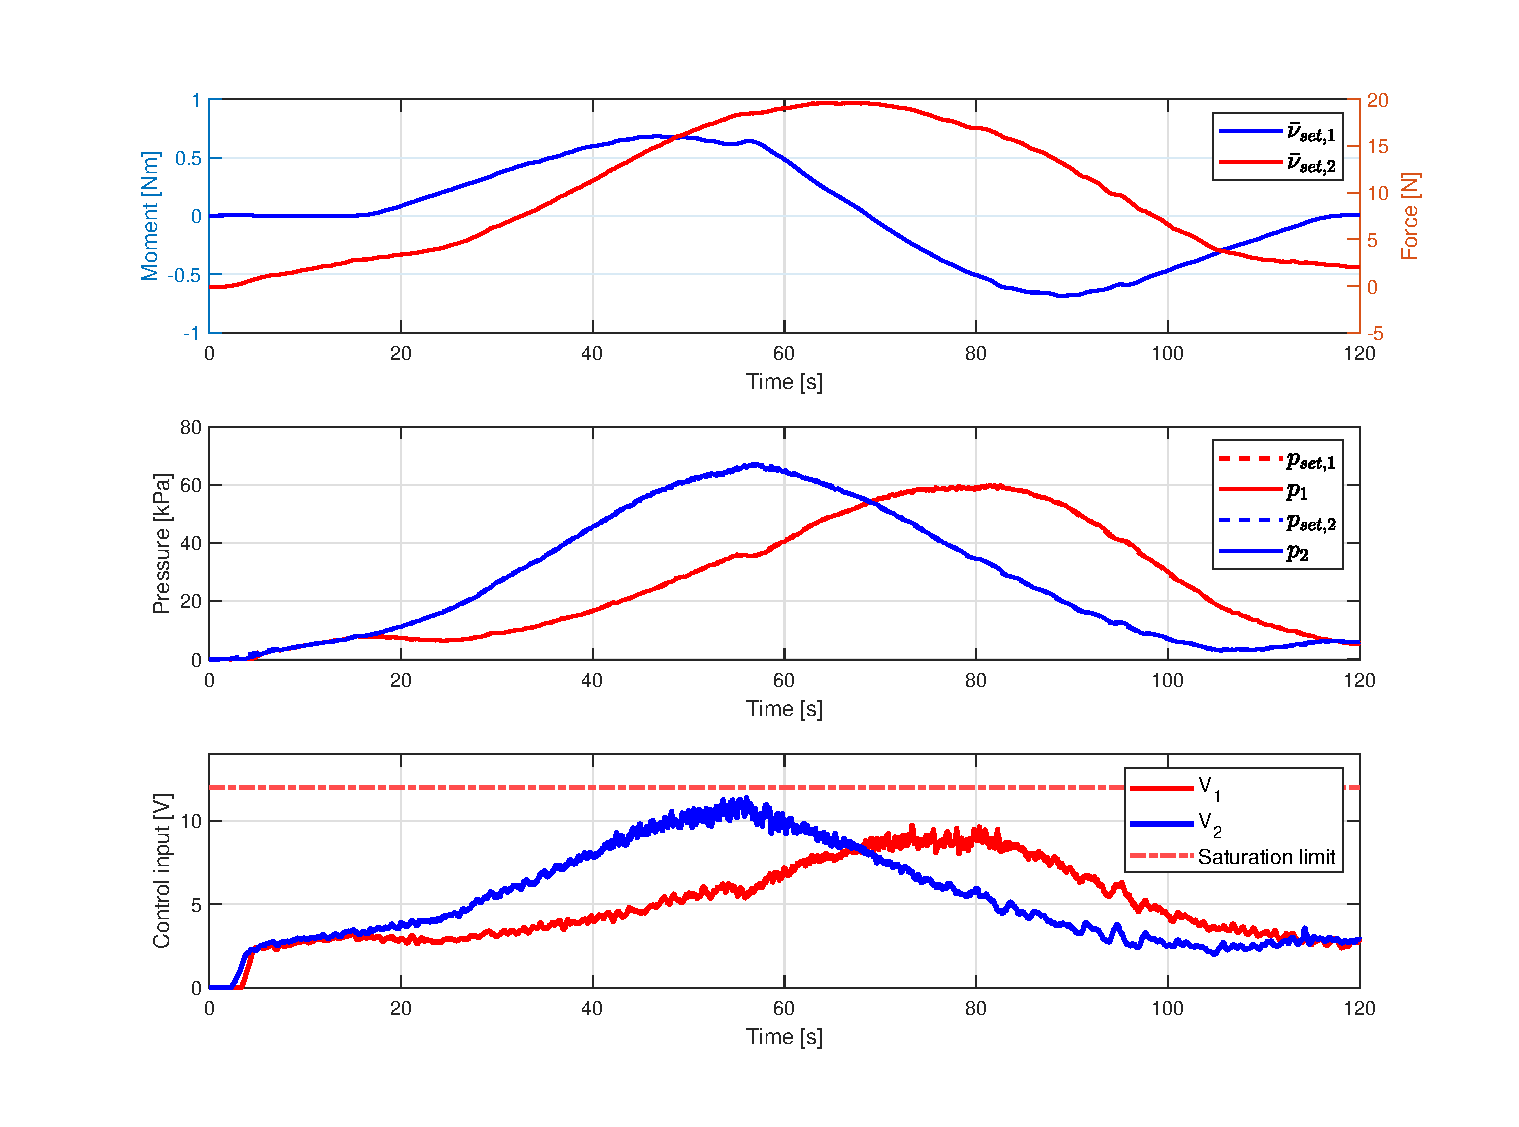
\includegraphics[width = \textwidth]{Figures/Chapter5/input.eps}
    \caption{\textbf{Top:} Control signal of model-based controller. \textbf{Middle:} Reference pressure and measured pressure. \textbf{Bottom:} Control input to the air pumps.}
    \label{fig5:controlellips}
\end{figure}

The errors in the bottom left and right quadrant of the ellipsoid are caused by a change in angular rate. Consider Figure \ref{fig5:ellipstheta} which shows the angle as function of time. Especially between 28 to 36 and 50 to 60 seconds the rotation data is inaccurate. This measurements is directly observed in the calculated end-effector position in the x,y plane. Since the angle data is used to calculate the end-effector position. This effect, together with the already observed noise deteriorates position calculation. In Figure \ref{fig5:ellipstheta} the effects of the sign change for the rotation are observed as spikes in the x and y position.

Furthermore, the effect on non-symmetrical material properties can be observed in Figure \ref{fig5:errorellips}. In the first halve of the ellipse the x-position is positive. During this 40 second period the actual position tends to be within the ellipsoid reference signal instead of on or outside the reference signal. For the second halve, the tracking is more accurate with errors both inside and outside the ellipsoid reference. Since the task-space has not been determined it remains hard to tell if the entire ellipsoid is situated in the robots task-space. 



\begin{figure}[H] 
    \begin{minipage}[b]{0.49\linewidth}
    \centering
    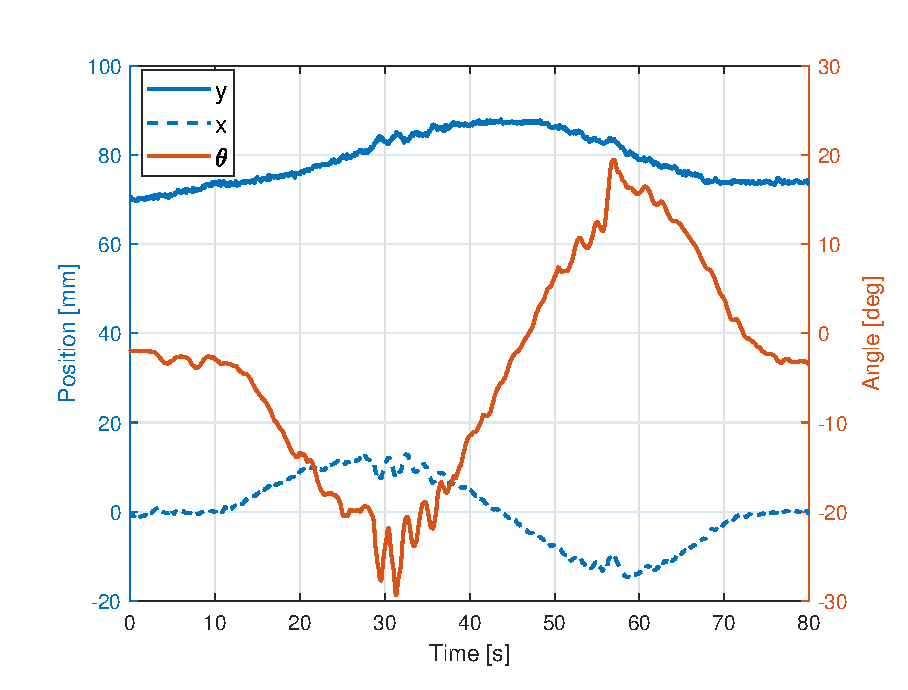
\includegraphics[width = \textwidth]{Figures/Chapter5/ellipsthetaxyh.eps}
    \caption{Angle $\theta$ and position in x and y direction as function of time.}
    \label{fig5:ellipstheta}
       \end{minipage} 
    \begin{minipage}[b]{0.49\linewidth}
    \centering
    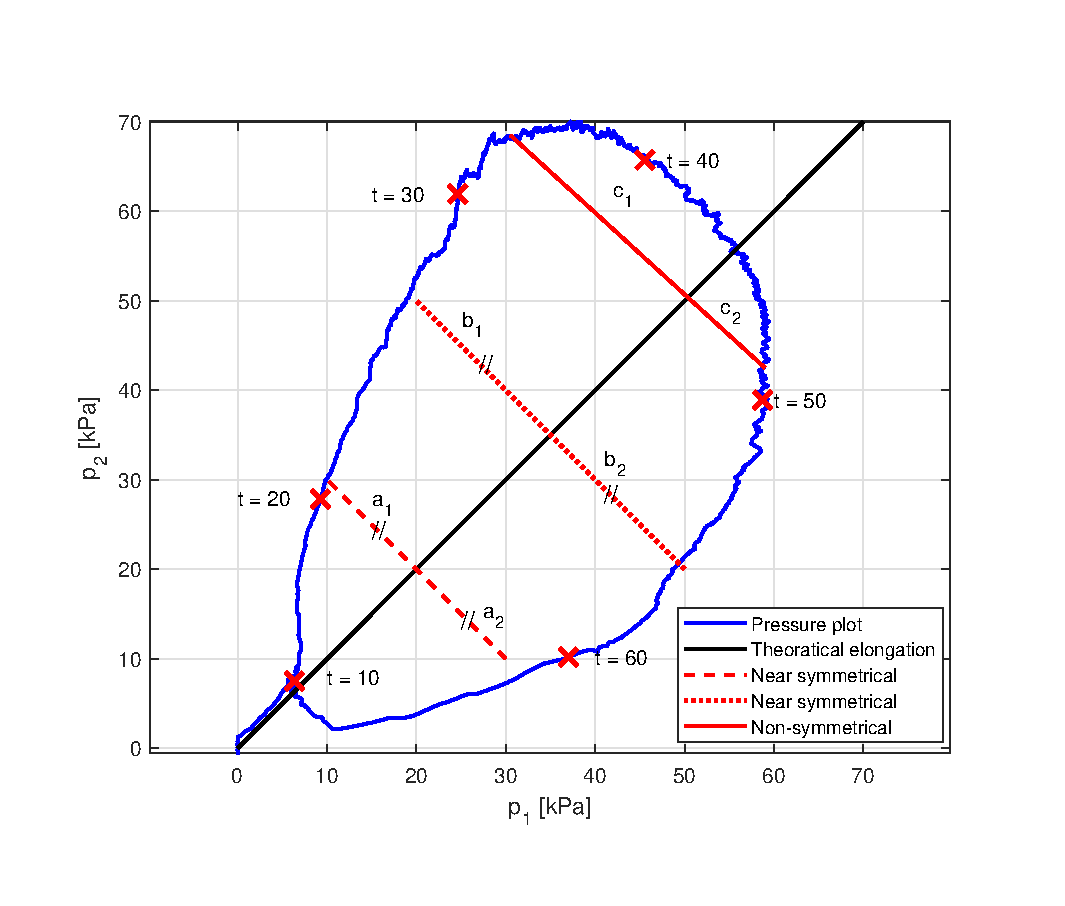
\includegraphics[width = \textwidth]{Figures/Chapter5/pressurecontour.eps}
    \caption{Contour plot of the bellow pressure $p_1$ and $p_2$.}
    \label{fig5:pressureellips}
    \end{minipage} 
\end{figure}

The unsymmetrical material properties are visualized by a pressure contour plot, as depicted in Figure \ref{fig5:pressureellips}. In this figure, the red crosses indicate time stamps. The solid black line indicates the pressures at which the actuator should theoretically only elongate. Perpendicular to this black line, red lines mark elongation and curvature set-points. Previously, it was assumed that the soft robot deforms symmetrically during rotation. However, this statement holds up til a pressure of about 50 kPa. The red lines $a_1$ and $a_2$ are of equal lengths and are close to measured pressures. This also holds for the lines $b_1$ and $b_2$. Considering pressures above 50 kPa, the symmetry argument does not hold. The lines $c_1$ and $c_2$ are not of equal length, indicating that curvature stiffness is dependent on the sign of the x-coordinate. 



\section{Model comparison to experimental results}

A qualitative comparison between the simulation and experimental results can not be drawn. However, some similarities and differences can be explained. 

First of all, the model and experimental results show similar behaviour. The step response's are difficult to compare regarding settling times and controller gains as a different input mapping was used. However, the general behaviour of the controller is similar. First, a step like control input to the air pumps is initiated, causing the actuator to rapidly move to the reference direction. Then a dip in control input is observed. From that point onwards the integrator gains cause the system to move to its desired position. In the experiments, a difference was observed for the mirrored set-points. This phenomenon is most likely to be caused by unequal pump characteristics. For the simulation, equal pump characteristics were assumed. 

Reference tracking in simulation and experiments show equal characteristics. The largest difference is the time in which the ellipsoid reference path was tracked. The actual system was able to track the ellipse in 100 seconds with an RMS error of ... and ... . For the model the time to complete the ellipsoid was set to 400 seconds. In simulation, an RMS error of $e_x = 0.1489 mm^2$ and $e_y = 0.0899 mm^2$ was found. Lowering the time to complete the ellipsoid is possible, at the cost of an increased error. A weigh-off is made between error and tracking speed. Currently, the low-pass filter of the model-based controller is $<0.1$ for simulation and experiments. This largely affects the control bandwidth but deemed necessary to reduce oscillations. 
